% !TEX program = xelatex
\documentclass[11pt,a4paper]{article}

\usepackage[a4paper,margin=2.3cm,headheight=14pt]{geometry}
\usepackage{fontspec}
\usepackage{amsmath,amssymb}
\usepackage[dvipsnames,table]{xcolor}

% ---------- colours ----------
\definecolor{acnavy}{RGB}{26,54,93}
\definecolor{acgreen}{RGB}{30,110,60}
\definecolor{acamber}{RGB}{214,137,16}
\definecolor{acplum}{RGB}{110,50,140}
\definecolor{acteal}{RGB}{0,120,125}

\usepackage{tikz}
\usetikzlibrary{arrows.meta,positioning,calc,shapes.geometric,fit,backgrounds}
\usepackage[most]{tcolorbox}
\usepackage{booktabs,array,tabularx,multirow,xltabular}
\usepackage{enumitem}
\usepackage{titlesec}
\usepackage{fancyhdr}
\usepackage{microtype}
\usepackage[colorlinks=true,linkcolor=acnavy,urlcolor=acnavy,citecolor=acnavy,
  pdftitle={Basics of Accounting -- Part 2: Terms, Principles, Concepts and Conventions},
  pdfsubject={Financial Analysis Course}]{hyperref}

% ---------- rupee symbol (font fallback) ----------
\newfontfamily\rsfont{DejaVu Sans}
\newcommand{\Rs}{\ifmmode\text{\rsfont ₹}\else{\rsfont ₹}\fi}

% ---------- layout ----------
\setlength{\parindent}{0pt}
\setlength{\parskip}{5pt plus 1pt}
\linespread{1.07}
\setlist{itemsep=2pt,topsep=4pt,parsep=0pt}
\renewcommand{\arraystretch}{1.3}
\newcolumntype{Y}{>{\raggedright\arraybackslash}X}
\setcounter{tocdepth}{2}

\titleformat{\section}{\Large\bfseries\sffamily\color{acnavy}}{\thesection}{0.7em}{}[{\color{acnavy}\titlerule[0.8pt]}]
\titleformat{\subsection}{\large\bfseries\sffamily\color{acnavy!85!black}}{\thesubsection}{0.6em}{}
\titleformat{\subsubsection}{\normalsize\bfseries\sffamily\color{acgreen}}{\thesubsubsection}{0.6em}{}
\titlespacing*{\section}{0pt}{18pt}{8pt}
\titlespacing*{\subsection}{0pt}{12pt}{4pt}
\titlespacing*{\subsubsection}{0pt}{8pt}{2pt}

\pagestyle{fancy}
\fancyhf{}
\fancyhead[L]{\small\sffamily\color{gray}Basics of Accounting --- Part 2}
\fancyhead[R]{\small\sffamily\color{gray}\leftmark}
\fancyfoot[C]{\small\sffamily\thepage}
\renewcommand{\headrulewidth}{0.3pt}

% ---------- coloured boxes ----------
\tcbset{boxstyle/.style={enhanced,breakable,arc=2pt,boxrule=0.6pt,
  left=8pt,right=8pt,top=6pt,bottom=6pt,
  fonttitle=\bfseries\sffamily\small,before skip=8pt,after skip=10pt}}
\newtcolorbox{defbox}[1]{boxstyle,colback=acnavy!5,colframe=acnavy,title={Definition: #1}}
\newtcolorbox{keybox}{boxstyle,colback=acgreen!6,colframe=acgreen,title={Key Idea}}
\newtcolorbox{impbox}[1][Important]{boxstyle,colback=acamber!9,colframe=acamber,title={#1}}
\newtcolorbox{exbox}[1]{boxstyle,colback=acplum!5,colframe=acplum,title={Example: #1}}
\newtcolorbox{casebox}[1]{boxstyle,colback=acteal!6,colframe=acteal,title={Case Study: #1}}
\newtcolorbox{notebox}[1][Note]{boxstyle,colback=gray!8,colframe=gray!70,title={#1}}

% ---------- TikZ styles ----------
\tikzset{
  stage/.style={draw=acnavy,fill=acnavy!10,rounded corners=3pt,minimum width=1.9cm,
    minimum height=1.0cm,align=center,font=\sffamily\scriptsize\bfseries},
  flowbox/.style={draw=acnavy,fill=acnavy!10,rounded corners=3pt,minimum height=0.95cm,
    align=center,font=\sffamily\small\bfseries,inner sep=5pt},
  outbox/.style={draw=acgreen,fill=acgreen!10,rounded corners=3pt,minimum height=0.95cm,
    align=center,font=\sffamily\small\bfseries,inner sep=5pt},
  arr/.style={-{Stealth[length=2mm]},thick,acnavy},
  capt/.style={font=\sffamily\tiny,text width=1.9cm,align=center,text=black!70}
}


% ---------- extra helpers for Part 2 ----------
\tikzset{
  lvl0/.style={draw=acnavy,fill=acnavy!15,rounded corners=3pt,font=\sffamily\bfseries\small,minimum width=3cm,minimum height=0.9cm,align=center,inner sep=4pt},
  lvl1/.style={draw=acgreen,fill=acgreen!10,rounded corners=3pt,font=\sffamily\footnotesize\bfseries,text width=3.3cm,minimum height=1.0cm,align=center,inner sep=4pt},
  lvl2/.style={draw=acamber,fill=acamber!12,rounded corners=3pt,font=\sffamily\scriptsize,text width=3.4cm,minimum height=1.1cm,align=center,inner sep=4pt}
}
\newcommand{\partheader}[3]{%
  \clearpage
  \addcontentsline{toc}{part}{#1: #2}%
  \markboth{#1}{#1}%
  \begin{tcolorbox}[enhanced,colback=acnavy,colframe=acnavy,arc=3pt,left=14pt,right=14pt,top=12pt,bottom=12pt,before skip=0pt,after skip=14pt]
    {\color{white}\sffamily{\small\bfseries #1}\\[3pt]{\LARGE\bfseries #2}\\[4pt]{\small #3}}
  \end{tcolorbox}%
}
\begin{document}

% =====================================================================
%                              TITLE PAGE
% =====================================================================
\begin{titlepage}
\thispagestyle{empty}
\begin{tikzpicture}[remember picture,overlay]
  \fill[acnavy] (current page.north west) rectangle ($(current page.north east)+(0,-12.6cm)$);
  \fill[acamber] ($(current page.north west)+(0,-12.6cm)$) rectangle ($(current page.north east)+(0,-12.9cm)$);
\end{tikzpicture}
\vspace*{1.6cm}
{\color{white}\sffamily
{\large\bfseries FINANCIAL ANALYSIS COURSE \ $\cdot$ \ STUDY NOTES}\\[1.3cm]
{\fontsize{36}{42}\selectfont\bfseries Basics of\\[2pt]Accounting}\\[0.6cm]
{\fontsize{19}{23}\selectfont Part 2: Basic Accounting Terms,\\[2pt] Principles, Concepts and Conventions}\\[0.7cm]
{\large Capital $\cdot$ Liabilities $\cdot$ Assets $\cdot$ Expenditure and Income\\
Trade Terms $\cdot$ Discounts $\cdot$ Accounting Concepts $\cdot$ Conventions}}
\vfill
{\sffamily
\begin{tcolorbox}[enhanced,colback=white,colframe=acnavy!40,boxrule=0.5pt,arc=3pt]
\textbf{What these notes are.} A detailed, explanatory rewrite of the lecture notes on
\emph{Basics of Accounting} Parts 2\_A, 2\_B and 2\_C. They continue directly from Part 1
(meaning, functions and cycle of accounting). Every idea in the lecture notes is covered, in
sequence, with definitions, formulas, worked examples and case studies, followed by an
integrated case study, a glossary, revision sheets and a self-test.
\end{tcolorbox}}
\vspace{0.6cm}
\begin{center}\sffamily\color{gray} October 2026\end{center}
\end{titlepage}

% =====================================================================
%                         ABOUT / HOW TO USE
% =====================================================================
\section*{About These Notes}
\addcontentsline{toc}{section}{About These Notes}
\markboth{About These Notes}{About These Notes}

\subsection*{What Part 2 covers and why it matters}
Part 1 explained what accounting is and how transactions flow through the accounting cycle. Part 2
supplies the \textbf{vocabulary and the rulebook} that every later topic depends on. Those later
topics (the accounting equation, the rules of debit and credit, journal entries, the ledger and
the trial balance) cannot be understood without the terms and principles below.

\begin{center}
\footnotesize\renewcommand{\arraystretch}{1.08}
\begin{tabularx}{\textwidth}{@{}l Y l@{}}
\toprule
\rowcolor{acnavy!15}\textbf{Part} & \textbf{Content} & \textbf{Lecture}\\
\midrule
\textbf{I} & Capital, drawings, liabilities (and their classification), business transaction vs.\ event, assets (and their classification), how capital, assets and liabilities relate & 2\_A\\
\textbf{II} & Expenditure (capital vs.\ revenue), expense, prepaid and outstanding expenses, income, revenue, profit, gain, loss, purchases, sales, returns, stock, inventory, bills, debtors, creditors, bad debts, insolvency, trade and cash discount & 2\_B\\
\textbf{III} & Accounting principles and GAAP; eight accounting concepts; four accounting conventions & 2\_C\\
\textbf{IV} & Integrated case study, glossary, revision sheets, self-test with answers & all\\
\bottomrule
\end{tabularx}
\end{center}

\subsection*{Colour-coded boxes}
\begingroup\small\tcbset{boxstyle/.append style={before skip=3pt,after skip=3pt,top=2pt,bottom=2pt}}
\begin{defbox}{Blue box}
Formal definitions. Learn these word for word.
\end{defbox}
\begin{keybox}
Green box: the one-line takeaway of a topic, often the question the topic answers.
\end{keybox}
\begin{impbox}
Amber box: rules, warnings, traps, and ``modern terminology'' clarifications.
\end{impbox}
\begin{exbox}{Purple box}
Worked examples with numbers.
\end{exbox}
\begin{casebox}{Teal box}
Case studies that tie several ideas together.
\end{casebox}
\begin{notebox}[Conventions]
Amounts are in Indian Rupees (\Rs) with Indian digit grouping (\Rs 5,00,000 is five lakh). Where an
example is not from the lecture notes, its assumptions are stated openly.
\end{notebox}
\endgroup

\clearpage
\tableofcontents
\clearpage

% =====================================================================
%                              PART I  (2_A)
% =====================================================================
\partheader{Part I \ (Lecture 2\_A)}{Capital, Drawings, Liabilities and Assets}{The terms that describe what a business owns, what it owes, and what belongs to its owner}

\section{Basic Accounting Terms: Where This Fits}

This lecture begins the next major section of the course, \textbf{Basic Accounting Terms}. These terms
are essential because later topics depend on understanding them precisely. The sequence indicated in
the course material is:

\begin{center}
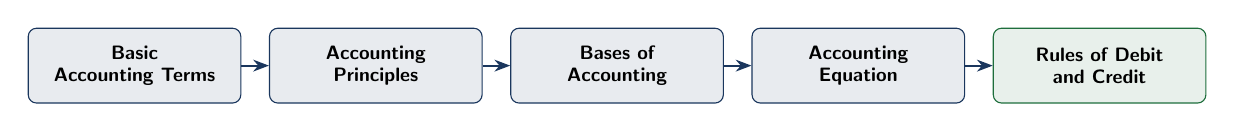
\begin{tikzpicture}[node distance=0.35cm]
  \node[flowbox,minimum width=2.7cm,font=\sffamily\scriptsize\bfseries] (a) {Basic\\Accounting Terms};
  \node[flowbox,minimum width=2.7cm,font=\sffamily\scriptsize\bfseries,right=of a] (b) {Accounting\\Principles};
  \node[flowbox,minimum width=2.7cm,font=\sffamily\scriptsize\bfseries,right=of b] (c) {Bases of\\Accounting};
  \node[flowbox,minimum width=2.7cm,font=\sffamily\scriptsize\bfseries,right=of c] (d) {Accounting\\Equation};
  \node[outbox,minimum width=2.7cm,font=\sffamily\scriptsize\bfseries,right=of d] (e) {Rules of Debit\\and Credit};
  \foreach \x/\y in {a/b,b/c,c/d,d/e} \draw[arr] (\x) -- (\y);
\end{tikzpicture}
\end{center}

\begin{notebox}[Where each step is covered in these notes]
\textbf{Basic accounting terms} are Parts I and II below (lectures 2\_A and 2\_B).
\textbf{Accounting principles} are Part III (lecture 2\_C). Bases of accounting, the accounting
equation (introduced informally here) and the debit--credit rules come in the following lectures.
\end{notebox}

\textbf{Part I} introduces four families of terms: \emph{capital}, \emph{drawings}, \emph{liabilities}
and \emph{assets}. It also separates a \emph{business transaction} from an \emph{event}.

% =====================================================================
\section{Capital}

\subsection{Meaning}

\begin{defbox}{Capital}
\textbf{Capital} is the amount invested by the proprietor (owner) in a business. It represents the
\textbf{owner's financial interest} in the business.
\end{defbox}

Capital may also be described as:
\begin{itemize}
  \item \textbf{Owner's equity},
  \item \textbf{Net worth},
  \item \textbf{Net assets}.
\end{itemize}

At a basic level capital is what is left for the owner after the business has covered its
obligations to outsiders:

\[
\boxed{\text{Capital}=\text{Assets}-\text{Liabilities}}
\qquad\Longleftrightarrow\qquad
\boxed{\text{Assets}=\text{Liabilities}+\text{Capital}}
\]

The second form is the \textbf{basic accounting equation} as given in this lecture.

\begin{exbox}{Owner starts a business}
The owner starts a business by investing \Rs 5,00,000 in cash. Then assets (cash) rise by
\Rs 5,00,000 and capital rises by \Rs 5,00,000:
\[
\text{Assets}=\Rs\,5{,}00{,}000,\qquad \text{Liabilities}=\Rs\,0,\qquad \text{Capital}=\Rs\,5{,}00{,}000,
\]
\[
\Rs\,5{,}00{,}000=\Rs\,0+\Rs\,5{,}00{,}000 .
\]
\end{exbox}

\subsection{Capital as the owner's claim}

Capital is not simply ``cash put into the business''. Once the money is invested, the \emph{business}
owns the resulting resources, while the \emph{owner} has a \textbf{claim (equity interest)} in the net
assets of the business.

\begin{exbox}{Cash turned into machinery}
An owner contributes \Rs 10 lakh and the business uses it to buy machinery. The owner's capital is
\emph{still} \Rs 10 lakh initially. What has changed is the \textbf{form of the business's assets}
(from cash to machinery), not the owner's claim.
\end{exbox}

\begin{keybox}
Capital is a \textbf{claim}, not a particular asset. The assets may change form many times while the
owner's claim stays the same, until profit, loss, drawings or additional investment change it.
\end{keybox}

% =====================================================================
\section{Drawings}

\subsection{Meaning}

\begin{defbox}{Drawings}
\textbf{Drawings} are cash, goods or other business resources withdrawn by the owner for
\textbf{personal use or private purposes}.
\end{defbox}

\textbf{Examples}
\begin{itemize}
  \item The owner withdraws \Rs 20,000 cash for personal expenses.
  \item The owner takes inventory worth \Rs 5,000 home for personal use.
  \item The business pays a personal expense of the owner.
\end{itemize}

These withdrawals \textbf{reduce the owner's equity} in the business.

\subsection{Relationship with capital}

\[
\boxed{\text{Closing Capital}=\text{Opening Capital}+\text{Profit}-\text{Drawings}+\text{Additional Capital}}
\]

\begin{impbox}[Drawings are not a business expense]
Drawings are \textbf{not} an expense in the usual sense. They are a \textbf{withdrawal of the owner's
interest} from the business. They therefore do not enter the calculation of profit; they are deducted
from the owner's capital instead.
\end{impbox}

\begin{exbox}{Effect of drawings}
Opening capital \Rs 5,00,000; drawings \Rs 50,000. Ignoring profit and additional capital:
\[
\text{Closing Capital}=5{,}00{,}000-50{,}000=\Rs\,4{,}50{,}000 .
\]
\end{exbox}

\begin{center}
\small
\begin{tabularx}{\textwidth}{@{}l Y Y@{}}
\toprule
\rowcolor{acnavy!15}\textbf{Item} & \textbf{Effect on owner's equity} & \textbf{Why}\\
\midrule
Additional capital introduced & Increases & Owner puts more into the business\\
Profit for the period & Increases & Business has earned more than it spent\\
Loss for the period & Decreases & Business has spent more than it earned\\
Drawings & Decreases & Owner takes resources out for private use\\
\bottomrule
\end{tabularx}
\end{center}

% =====================================================================
\section{Liabilities}

\subsection{Meaning}

\begin{defbox}{Liability}
A \textbf{liability} is an amount or obligation that the business \textbf{owes to outsiders} or
otherwise has an obligation to settle.
\end{defbox}

\textbf{Examples:} loans, creditors (trade payables), outstanding wages, outstanding expenses and
other financial obligations.

\[
\boxed{\text{Liability}=\text{Amount or obligation owed by the business}}
\]

\begin{exbox}{Bank loan}
The business borrows \Rs 2,00,000 from a bank. It receives \Rs 2,00,000 in cash, but at the same time
has an \textbf{obligation to repay the bank}. Therefore \text{Liability}~$=\Rs\,2{,}00{,}000$.
\end{exbox}

% =====================================================================
\section{Classification of Liabilities}

The lecture classifies liabilities in two different ways. The two systems answer \emph{different
questions}.

\begin{center}
\small
\begin{tabularx}{\textwidth}{@{}l Y Y@{}}
\toprule
\rowcolor{acnavy!15}\textbf{Basis} & \textbf{Question answered} & \textbf{Categories}\\
\midrule
\textbf{A. To whom payable} & Who is the claimant? & Internal liabilities; external liabilities\\
\textbf{B. When payable} & How soon must it be settled? & Current liabilities; non-current liabilities\\
\bottomrule
\end{tabularx}
\end{center}

\subsection{Internal liabilities}

In the terminology of the lecture, \textbf{internal liabilities} are amounts attributable to the
\textbf{proprietor / owner(s)}. In basic accounting the owner's claim is represented by
\textbf{capital / equity}, so the lecture uses ``internal liability'' for the amount the business
owes or attributes to its owners.

\begin{exbox}{Internal liability}
Owner's capital of \Rs 1,00,000 represents the owner's claim on the business.
\end{exbox}

\begin{impbox}[Modern terminology]
In contemporary financial reporting the owner's claim is classified as \textbf{equity}, not as a
liability to external creditors.
\[
\boxed{\text{Owner's claim}=\text{Equity}}\qquad\qquad\boxed{\text{External obligations}=\text{Liabilities}}
\]
\end{impbox}

\subsection{External liabilities}

\textbf{External liabilities} are obligations that the business owes to \textbf{outsiders}. Examples:
bank loans, trade creditors, outstanding expenses and other amounts payable.

\begin{exbox}{Supplier on credit}
The business owes \Rs 75,000 to a supplier for goods purchased on credit. Trade payable $=\Rs\,75{,}000$.
It is an external obligation because it is payable to a party outside the ownership of the business.
\end{exbox}

\subsection{Current and non-current liabilities}

This classification is based on \textbf{maturity (payment period)}.

\begin{center}
\small
\begin{tabularx}{\textwidth}{@{}l Y Y@{}}
\toprule
\rowcolor{acnavy!15} & \textbf{Current liabilities} & \textbf{Non-current liabilities}\\
\midrule
\textbf{Meaning} & Obligations expected to be settled within the short-term operating cycle, or generally \textbf{within one year} & Obligations \emph{not} expected to be settled within the current short-term period, commonly those payable \textbf{after more than one year}\\
\textbf{Lecture's simple rule} & Liabilities to be paid within 1 year & Liabilities to be paid after more than 1 year\\
\textbf{Examples} & Trade payables, short-term borrowings, outstanding salaries, outstanding expenses, other short-term obligations & Long-term bank loans, long-term borrowings, long-term debt obligations\\
\bottomrule
\end{tabularx}
\end{center}

\begin{impbox}[A note on the one-year rule]
The precise definition of ``current liability'' under formal accounting standards can involve conditions
beyond simply ``one year''. For this introductory course the one-year distinction is the useful basic rule.
\end{impbox}

\subsection{Case study: classifying liabilities}

\begin{casebox}{Mr.\ X}
Mr.\ X invests \Rs 10,000 in his business and takes a loan of \Rs 25,000 from SBI Bank for
\textbf{10 years}. He then purchases goods worth \Rs 2,000 from Mr.\ Y on credit for \textbf{2 months}.
Classify each amount.

\medskip
\textbf{Transaction 1: owner invests \Rs 10,000.} This is the owner's contribution, so
Capital / Owner's equity $=\Rs\,10{,}000$. In the lecture's terminology it is an \emph{internal
liability}; in modern accounting it is \emph{equity}.

\textbf{Transaction 2: SBI loan of \Rs 25,000 for 10 years.} The business owes the bank, so it is an
\textbf{external} liability. It is due over 10 years, so it is a \textbf{non-current} liability.

\textbf{Transaction 3: credit purchase of \Rs 2,000 from Mr.\ Y for 2 months.} The business owes
Mr.\ Y, so it is an \textbf{external} liability. It is payable within 2 months, so it is a
\textbf{current} liability.

\begin{center}
\small
\begin{tabularx}{\textwidth}{@{}Y r Y@{}}
\toprule
\rowcolor{acteal!15}\textbf{Item} & \textbf{Amount} & \textbf{Classification}\\
\midrule
Owner's investment & \Rs 10,000 & Capital / equity (lecture term: internal liability)\\
SBI Bank loan & \Rs 25,000 & External $+$ non-current liability\\
Credit purchase from Mr.\ Y & \Rs 2,000 & External $+$ current liability\\
\bottomrule
\end{tabularx}
\end{center}
\end{casebox}

\begin{keybox}
The same liability carries \textbf{two classifications at once}, one from each system, for example
\emph{External $+$ Current} or \emph{External $+$ Non-current}, because the two systems measure different
dimensions (\emph{who} is owed, \emph{when} it is due).
\end{keybox}

\subsubsection{The two classifications side by side}

\begin{center}
\small
\begin{tabularx}{\textwidth}{@{}l Y Y@{}}
\toprule
\rowcolor{acnavy!15} & \textbf{Current (due within 1 year)} & \textbf{Non-current (due after 1 year)}\\
\midrule
\textbf{External (owed to outsiders)} & Trade payables, outstanding expenses, short-term loans & Long-term bank loan (e.g.\ the SBI loan)\\
\textbf{Internal (owner's claim)} & --- & Capital / equity (in modern terms, equity is not a liability at all)\\
\bottomrule
\end{tabularx}
\end{center}

% =====================================================================
\section{Business Transaction versus Event}

The lecture introduces an important conceptual distinction.

\subsection{Business transaction}

\begin{defbox}{Business transaction (as defined in this lecture)}
A \textbf{business transaction} is an economic activity of the business that \textbf{changes its
financial position} and can be \textbf{expressed in monetary terms}.
\end{defbox}

It therefore has (1) a financial effect on the business and (2) a measurable monetary value.
Examples: purchase of goods, sale of goods, purchase of machinery, payment of salary, receipt of cash,
borrowing from a bank.

\subsection{Event}

An \textbf{event} is the \textbf{result or consequence of a transaction}.

\begin{exbox}{Purchase and sale}
Goods are purchased for \Rs 2 lakh and sold for \Rs 2.5 lakh.

\textbf{Transactions:} (1) purchase of goods for \Rs 2 lakh; (2) sale of goods for \Rs 2.5 lakh.

\textbf{Event / result:} the difference, $2.5-2=\Rs\,0.5$ lakh, so \textbf{Profit $=\Rs\,50{,}000$}.
The lecture calls this profit the \emph{event (result) arising from the transactions}.
\end{exbox}

\[
\text{Business transactions}\;\rightarrow\;\text{Changes in accounts}\;\rightarrow\;\text{Financial result}
\]

So transactions are the economic activities, and events or results may arise from them.

\begin{impbox}[A broader meaning of ``event'']
In broader accounting terminology, ``event'' can have a \textbf{wider meaning} than the narrow definition
in the lecture. It may include any economic occurrence that affects the financial statements even when it
is not a conventional exchange transaction. For this course remember the lecture's distinction, while
keeping the wider meaning in mind.
\end{impbox}

\begin{notebox}[Link to Part 1]
In Part 1 a business transaction was an economic event that is measurable in money and has a financial effect
on the business. The two definitions agree. Part 2 adds that the \emph{result} of transactions (such as profit)
is called an event.
\end{notebox}

% =====================================================================
\section{Assets}

\subsection{Meaning}

\begin{defbox}{Asset}
An \textbf{asset} is a valuable \textbf{economic resource controlled by a business} as a result of
\textbf{past events}, from which \textbf{future economic benefits} are expected.
\end{defbox}

The lecture gives a simpler formulation: \emph{assets are valuable resources owned by businesses that are
acquired at a measurable monetary cost.} Examples given: cash, land, furniture. Others: buildings, machinery,
inventory, trade receivables, vehicles, computers.

\subsection{Important characteristics of assets}

\begin{center}
\small
\begin{tabularx}{\textwidth}{@{}c l Y@{}}
\toprule
\rowcolor{acnavy!15}\textbf{\#} & \textbf{Characteristic} & \textbf{Explanation}\\
\midrule
1 & Provides economic value & The resource has the capacity to provide future economic benefits\\
2 & Controlled by the business & The business must have control over the resource\\
3 & Arises from a past event or transaction & For example, a machine that was purchased earlier\\
4 & Can be recognised and measured & It must satisfy the applicable recognition and measurement requirements\\
\bottomrule
\end{tabularx}
\end{center}

% =====================================================================
\section{Classification of Assets}

The lecture divides assets into \textbf{three broad categories}:
\begin{enumerate}
  \item \textbf{Non-current assets},
  \item \textbf{Current assets},
  \item \textbf{Fictitious / nominal assets}.
\end{enumerate}
It also divides non-current assets into \textbf{tangible} and \textbf{intangible} assets.

\begin{center}
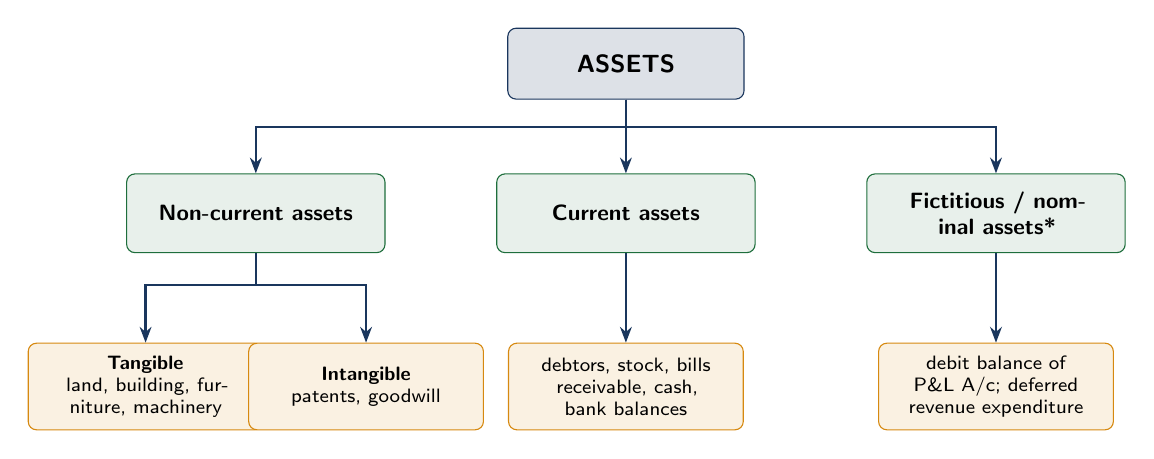
\begin{tikzpicture}
 \node[lvl0] (root) at (0,0) {ASSETS};
 \node[lvl1,text width=3.0cm] (nca) at (-4.7,-1.9) {Non-current assets};
 \node[lvl1,text width=3.0cm] (ca) at (0,-1.9) {Current assets};
 \node[lvl1,text width=3.0cm] (fa) at (4.7,-1.9) {Fictitious / nominal assets*};
 \node[lvl2,text width=2.7cm] (tan) at (-6.1,-4.1) {\textbf{Tangible}\\land, building, furniture, machinery};
 \node[lvl2,text width=2.7cm] (int) at (-3.3,-4.1) {\textbf{Intangible}\\patents, goodwill};
 \node[lvl2,text width=2.7cm] (cae) at (0,-4.1) {debtors, stock, bills receivable, cash, bank balances};
 \node[lvl2,text width=2.7cm] (fae) at (4.7,-4.1) {debit balance of P\&L A/c; deferred revenue expenditure};
 \draw[arr] (root.south) -- ++(0,-0.35) -| (nca.north);
 \draw[arr] (root.south) -- (ca.north);
 \draw[arr] (root.south) -- ++(0,-0.35) -| (fa.north);
 \draw[arr] (nca.south) -- ++(0,-0.4) -| (tan.north);
 \draw[arr] (nca.south) -- ++(0,-0.4) -| (int.north);
 \draw[arr] (ca.south) -- (cae.north);
 \draw[arr] (fa.south) -- (fae.north);
\end{tikzpicture}

{\footnotesize *Traditional accounting terminology; see Section~\ref{sec:fict}.}
\end{center}

\subsection{Non-current assets}

\begin{defbox}{Non-current assets}
Assets that are held for \textbf{continued use} in the business, particularly for producing goods or
rendering services, and are \textbf{not intended for resale in the ordinary course of business}.
\end{defbox}

\textbf{Examples given:} land, buildings, furniture. \textbf{Others:} plant and machinery, office equipment,
vehicles, computers used in operations.

\[
\boxed{\text{Non-current asset}=\text{Long-term resource used in the business}}
\]
(rather than inventory held primarily for sale).

\begin{exbox}{Use decides classification}
A furniture manufacturer has a machine used to make furniture. The machine is a \textbf{non-current asset}
because it is used to produce goods. The furniture manufactured for sale is generally \textbf{inventory}, a
current asset. Classification depends partly on \emph{how the resource is used} by the business.
\end{exbox}

\subsubsection{Tangible assets}

A \textbf{tangible asset} has a \textbf{physical existence}. Examples: land, buildings, furniture, machinery,
vehicles, computers. A computer used by an office is tangible because it has a physical form.
\[
\boxed{\text{Tangible}\Rightarrow\text{Physical form}}
\]

\subsubsection{Intangible assets}

An \textbf{intangible asset} does \textbf{not have a physical form} but may still provide economic benefits.
Examples given: patents, goodwill. Others: certain copyrights, trademarks, software rights or licences.
\[
\boxed{\text{Intangible}\Rightarrow\text{No physical substance}}
\]
A patent has no physical shape like machinery, but it provides economic benefits through legal rights.

\subsubsection{Tangible versus intangible}

\begin{center}
\small
\begin{tabularx}{\textwidth}{@{}l Y Y@{}}
\toprule
\rowcolor{acnavy!15}\textbf{Basis} & \textbf{Tangible assets} & \textbf{Intangible assets}\\
\midrule
Physical existence & Yes & No physical substance\\
Examples & Land, building, furniture, machinery & Patent, goodwill, certain copyrights and trademarks\\
Nature & Physical resources & Rights or benefits without physical form\\
\bottomrule
\end{tabularx}
\end{center}

\textbf{Memory trick.} \textbf{Tangible $=$ touchable.} \textbf{Intangible $=$ cannot be physically touched.}

\subsection{Current assets}

The lecture also calls current assets \textbf{floating assets} or \textbf{circulating assets}. They are
generally assets that are \textbf{held for sale}, or \textbf{expected to be converted into cash or consumed
in the short term} (commonly within one year in introductory classification).

\textbf{Examples:} debtors (trade receivables), stock (inventory), bills receivable, cash, bank balances, and
short-term investments in appropriate classifications.

Current assets are associated with the \textbf{normal operating cycle and short-term liquidity} of the business.

\subsubsection{Why ``circulating''?}

Because they continuously move through the operating cycle. For a trading business:

\begin{center}
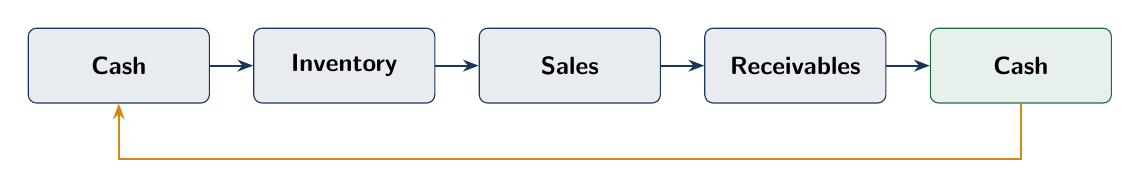
\begin{tikzpicture}[node distance=0.55cm]
  \node[flowbox,minimum width=2.3cm,font=\sffamily\small\bfseries] (c1) {Cash};
  \node[flowbox,minimum width=2.3cm,font=\sffamily\small\bfseries,right=of c1] (c2) {Inventory};
  \node[flowbox,minimum width=2.3cm,font=\sffamily\small\bfseries,right=of c2] (c3) {Sales};
  \node[flowbox,minimum width=2.3cm,font=\sffamily\small\bfseries,right=of c3] (c4) {Receivables};
  \node[outbox,minimum width=2.3cm,font=\sffamily\small\bfseries,right=of c4] (c5) {Cash};
  \foreach \x/\y in {c1/c2,c2/c3,c3/c4,c4/c5} \draw[arr] (\x) -- (\y);
  \draw[arr,acamber] (c5.south) -- ++(0,-0.7) -| (c1.south);
\end{tikzpicture}
\end{center}

The resources \textbf{circulate through the business}, which is why the older teaching term
``circulating assets'' is used.

\subsubsection{Example: current versus non-current}

A company has \Rs 10 lakh of machinery used for manufacturing, \Rs 3 lakh of inventory held for sale and
\Rs 2 lakh receivable from customers.

\begin{center}
\small
\begin{tabularx}{\textwidth}{@{}l r Y@{}}
\toprule
\rowcolor{acnavy!15}\textbf{Item} & \textbf{Amount} & \textbf{Classification}\\
\midrule
Machinery & \Rs 10 lakh & Non-current asset (tangible)\\
Inventory & \Rs 3 lakh & Current asset\\
Trade receivables & \Rs 2 lakh & Current asset\\
\bottomrule
\end{tabularx}
\end{center}

\begin{keybox}
The classification does not depend on how \emph{expensive} an item is, but on \textbf{how and for what
purpose it is held}.
\end{keybox}

\subsection{Fictitious / nominal assets}
\label{sec:fict}

\begin{defbox}{Fictitious (nominal) assets}
Items that are neither tangible nor intangible assets in the normal sense but represent
\textbf{losses or expenses that are yet to be written off}.
\end{defbox}

\textbf{Examples given:} debit balance of the Profit \& Loss Account; deferred revenue expenditure.

\begin{impbox}[Modern accounting clarification]
``Fictitious asset'' is a \textbf{traditional} accounting term. Such items generally do \textbf{not} meet
the modern conceptual definition of an asset, because they do not necessarily represent a controlled resource
from which future economic benefits are expected. Under modern standards think of them as
\emph{unamortised or deferred amounts, or losses, appearing on the asset side under older presentation},
not as genuine economic assets.
\[
\boxed{\text{Fictitious asset}\neq\text{genuine economic asset}}
\]
\end{impbox}

\textbf{Why the name ``fictitious''?} They may appear in a traditional balance sheet alongside assets, but
they do not represent ordinary resources such as cash, machinery, inventory or buildings. For instance, an
amount that is \emph{not immediately charged in full} to the profit and loss account under an older treatment may
have its unamortised balance shown on the balance sheet. That balance is described as a ``fictitious asset''.

\subsection{Overall classification of assets}

\begin{center}
\small
\begin{tabularx}{\textwidth}{@{}l Y Y@{}}
\toprule
\rowcolor{acnavy!15}\textbf{Category} & \textbf{Meaning} & \textbf{Examples}\\
\midrule
\textbf{I. Non-current assets} & Resources held for long-term use in the business; further split into \emph{tangible} and \emph{intangible} & Land, building, furniture, machinery; patents, goodwill\\
\textbf{II. Current assets} & Resources expected to be sold, consumed or converted into cash in the short term & Debtors, stock, bills receivable, cash, bank\\
\textbf{III. Fictitious assets} & Traditional term for certain deferred or unwritten-off losses or expenses; not genuine assets under modern concepts & Debit balance of P\&L; deferred revenue expenditure\\
\bottomrule
\end{tabularx}
\end{center}

% =====================================================================
\section{Assets, Liabilities and Capital Together}

\subsection{Assets versus liabilities}

\begin{center}
\small
\begin{tabularx}{\textwidth}{@{}l Y@{}}
\toprule
\rowcolor{acnavy!15}\textbf{Term} & \textbf{Meaning}\\
\midrule
\textbf{Asset} & What the business owns or controls, an economic resource\\
\textbf{Liability} & What the business owes or is obligated to settle\\
\bottomrule
\end{tabularx}
\end{center}

\begin{exbox}{Machinery bought with a bank loan}
A company buys machinery for \Rs 5 lakh by taking a bank loan. Immediately, \textbf{asset}: machinery
$=\Rs\,5{,}00{,}000$; \textbf{liability}: bank loan $=\Rs\,5{,}00{,}000$. Then
$\text{Assets}=\text{Liabilities}+\text{Equity}$ becomes $5{,}00{,}000=5{,}00{,}000+0$.
\end{exbox}

\subsection{The core relationship}

\[
\boxed{\text{Assets}=\text{Liabilities}+\text{Capital}}
\qquad
\boxed{\text{Capital}=\text{Assets}-\text{Liabilities}}
\]

Everything the business has obtained can broadly be financed by only two sources:
\begin{enumerate}
  \item \textbf{Owners' funds} $\rightarrow$ capital / equity;
  \item \textbf{Outsiders' funds} $\rightarrow$ liabilities.
\end{enumerate}

\[
\boxed{\text{Resources of business}=\text{Owners' claim}+\text{Outsiders' claims}}
\]

\begin{center}
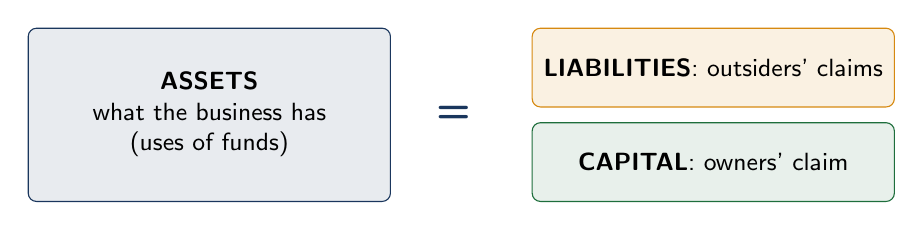
\begin{tikzpicture}
  \node[draw=acnavy,fill=acnavy!10,rounded corners=3pt,minimum width=4.6cm,minimum height=2.2cm,align=center,font=\sffamily\small] (A) at (0,0) {\textbf{ASSETS}\\what the business has\\(uses of funds)};
  \node[font=\sffamily\Large\bfseries,text=acnavy] at (3.1,0) {=};
  \node[draw=acamber,fill=acamber!12,rounded corners=3pt,minimum width=4.6cm,minimum height=1.0cm,align=center,font=\sffamily\small] (L) at (6.4,0.6) {\textbf{LIABILITIES}: outsiders' claims};
  \node[draw=acgreen,fill=acgreen!10,rounded corners=3pt,minimum width=4.6cm,minimum height=1.0cm,align=center,font=\sffamily\small] (C) at (6.4,-0.6) {\textbf{CAPITAL}: owners' claim};
\end{tikzpicture}
\end{center}

\subsection{Important relationships to remember}

\begin{center}
\small
\begin{tabularx}{\textwidth}{@{}l Y@{}}
\toprule
\rowcolor{acnavy!15}\textbf{Relationship} & \textbf{Statement}\\
\midrule
Capital & Capital $=$ Owner's equity\\
Net worth & Net worth $=$ Assets $-$ Liabilities\\
Accounting equation & Assets $=$ Liabilities $+$ Capital\\
Profit and capital & Profit $\uparrow\Rightarrow$ Equity $\uparrow$\\
Loss and capital & Loss $\uparrow\Rightarrow$ Equity $\downarrow$\\
Drawings and capital & Drawings $\uparrow\Rightarrow$ Equity $\downarrow$\\
\bottomrule
\end{tabularx}
\end{center}

\subsection{An integrated example}

\begin{exbox}{Four transactions and the equation}
\begin{enumerate}
  \item The owner invests \Rs 5,00,000: cash $+5{,}00{,}000$; capital $+5{,}00{,}000$.
  \item The business takes a \emph{long-term} bank loan of \Rs 2,00,000: cash $+2{,}00{,}000$; loan liability $+2{,}00{,}000$.
  \item Goods worth \Rs 1,00,000 are bought \emph{on credit}: inventory $+1{,}00{,}000$; trade payable $+1{,}00{,}000$. Total assets and total liabilities both rise by \Rs 1,00,000.
  \item The owner withdraws \Rs 20,000 cash: cash $-20{,}000$; drawings \Rs 20,000, so owner's equity falls by \Rs 20,000.
\end{enumerate}
\begin{center}
\small
\begin{tabularx}{\textwidth}{@{}l r r r Y@{}}
\toprule
\rowcolor{acplum!12}\textbf{After step} & \textbf{Assets} & \textbf{Liabilities} & \textbf{Capital} & \textbf{Check}\\
\midrule
1 & 5,00,000 & 0 & 5,00,000 & $5{,}00{,}000=0+5{,}00{,}000$\\
2 & 7,00,000 & 2,00,000 & 5,00,000 & $7{,}00{,}000=2{,}00{,}000+5{,}00{,}000$\\
3 & 8,00,000 & 3,00,000 & 5,00,000 & $8{,}00{,}000=3{,}00{,}000+5{,}00{,}000$\\
4 & 7,80,000 & 3,00,000 & 4,80,000 & $7{,}80{,}000=3{,}00{,}000+4{,}80{,}000$\\
\bottomrule
\end{tabularx}
\end{center}
(Amounts in \Rs; capital in step~4 is shown after deducting drawings. The step-wise totals are computed from
the lecture's four transactions.)
\end{exbox}

\subsection{Terminology cautions}

\begin{impbox}[Traditional versus modern usage]
\begin{itemize}
  \item \textbf{``Internal liability''}: traditional texts use it for the owner's claim. For modern clarity:
        the owner's claim is \textbf{equity}, not an external liability.
  \item \textbf{``Fictitious asset''}: a traditional term; do \textbf{not} read it as a genuine asset under modern concepts.
  \item \textbf{``Assets owned''}: a more precise modern idea is that an asset is a resource \textbf{controlled}
        by the entity, rather than merely something legally ``owned''.
\end{itemize}
\end{impbox}

\subsection{Quick revision table}

\begin{center}
\small
\begin{tabularx}{\textwidth}{@{}l Y Y@{}}
\toprule
\rowcolor{acnavy!15}\textbf{Term} & \textbf{Core meaning} & \textbf{Examples}\\
\midrule
\textbf{Capital} & Owner's investment or claim in the business & Owner invests cash\\
\textbf{Drawings} & Withdrawal of cash, goods or resources by the owner for personal use & Cash withdrawn for personal expenses\\
\textbf{Liability} & Obligation of the business & Loan, creditor\\
\textbf{Internal liability}$^{*}$ & Owner's claim in traditional terminology & Capital\\
\textbf{External liability} & Amount owed to outsiders & Bank loan, trade payable\\
\textbf{Current liability} & Short-term obligation & Trade payable, outstanding expense\\
\textbf{Non-current liability} & Long-term obligation & Long-term bank loan\\
\textbf{Asset} & Economic resource controlled by the business & Cash, land, machinery\\
\textbf{Non-current asset} & Long-term resource used in business & Machinery, building\\
\textbf{Tangible asset} & Asset with physical form & Furniture, computer\\
\textbf{Intangible asset} & Asset without physical form & Patent, goodwill\\
\textbf{Current asset} & Short-term operating or liquid resource & Inventory, receivables\\
\textbf{Fictitious asset}$^{*}$ & Traditional term for deferred or unwritten-off amounts & Debit balance of P\&L\\
\bottomrule
\end{tabularx}

{\footnotesize $^{*}$Traditional terminology; modern financial reporting may classify these differently.}
\end{center}

\subsection{Exam-oriented points for Part I}

\begin{defbox}{Capital}
The amount invested by the proprietor / owners in the business; it represents the owner's equity or residual
interest in the business.
\end{defbox}
\begin{defbox}{Drawings}
Cash, goods or other business resources withdrawn by the proprietor for personal or private purposes.
\end{defbox}
\begin{defbox}{Liability}
An obligation of the business to outsiders, or another obligation requiring settlement.
\end{defbox}
\begin{defbox}{Asset}
A resource controlled by the business as a result of past events, from which future economic benefits are expected.
\end{defbox}

\begin{center}
\small
\begin{tabularx}{\textwidth}{@{}l Y@{}}
\toprule
\rowcolor{acnavy!15}\textbf{Question} & \textbf{Answer in one line}\\
\midrule
State the accounting equation & Assets $=$ Liabilities $+$ Capital\\
Classify liabilities by claimant & Internal (owner's claim) and external\\
Classify liabilities by settlement period & Current and non-current\\
Classify assets & Non-current, current, and the traditional fictitious / nominal category\\
Classify non-current assets further & Tangible and intangible\\
\bottomrule
\end{tabularx}
\end{center}

\begin{keybox}
\textbf{Core takeaway of Part I.} A business's resources (\textbf{assets}) are financed by the claims of
\textbf{outsiders (liabilities)} and \textbf{owners (capital / equity)}: Assets $=$ Liabilities $+$ Capital.
Drawings reduce the owner's equity; liabilities are classified by \emph{whom} they are owed to and by
\emph{maturity}; and assets by \emph{use}, \emph{liquidity} and \emph{physical nature}.
\end{keybox}

% =====================================================================
%                              PART II  (2_B)
% =====================================================================
\partheader{Part II \ (Lecture 2\_B)}{Expenditure, Income and Trade Terms}{Expenditure, expense, income, revenue, profit, gain, loss; purchases, sales, stock, bills, debtors, creditors, bad debts and discounts}

\section{Introduction to Part II}

Part I introduced capital, drawings, liabilities and assets. Part II continues with another set of fundamental
terms:

\[
\boxed{\text{Expenditure, Expense, Income, Revenue, Profit, Gain, Loss}}
\]

and then moves to \textbf{trade-related terminology}: bills, debtors, creditors, bad debts, insolvency, discount,
stock and inventory.

\begin{impbox}[Why these terms need care]
Many of these words sound alike in everyday language but have \textbf{different meanings in accounting}
(expenditure vs.\ expense, revenue vs.\ gain, expense vs.\ loss, trade discount vs.\ cash discount). Each
pair is compared explicitly below.
\end{impbox}

% =====================================================================
\section{Expenditure}

\begin{defbox}{Expenditure}
\textbf{Expenditure} is a disbursement of cash, transfer of other property, or incurrence of a liability for the
purpose of acquiring \textbf{assets, goods or services}.
\end{defbox}

In simple terms: \emph{expenditure is the amount spent, or obligation incurred, to obtain something for the
business.}

\textbf{Examples:} purchasing machinery for \Rs 5,00,000; purchasing goods for resale for \Rs 1,00,000; paying
rent of \Rs 20,000; purchasing office supplies for \Rs 5,000. All involve expenditure.

\begin{impbox}[Expenditure does not automatically mean expense]
This is one of the most important distinctions in this chapter. An expenditure may result in
\textbf{an asset being acquired}, or \textbf{an expense being recognised}.
\end{impbox}

% =====================================================================
\section{Capital Expenditure versus Revenue Expenditure}

Expenditure is divided broadly into two kinds, based on the \textbf{nature and benefit} of the spending.

\[
\boxed{\text{Capital Expenditure}\quad\text{and}\quad\text{Revenue Expenditure}}
\]

\subsection{Capital expenditure}

\begin{defbox}{Capital expenditure}
Expenditure incurred to \textbf{acquire a long-term (permanent) asset} or to \textbf{improve an existing
long-term asset}, where the asset is \textbf{not intended for resale in the ordinary course of business}.
\end{defbox}

It can therefore increase the value or productive capacity of a business asset. Examples: purchase of machinery,
land or a building; major expenditure that improves the capacity of an existing machine.

\textbf{Key idea.} Capital expenditure is about \textbf{creating or improving a long-term productive resource}.

\subsubsection{Characteristics of capital expenditure}

\begin{center}
\small
\begin{tabularx}{\textwidth}{@{}c l Y@{}}
\toprule
\rowcolor{acnavy!15}\textbf{\#} & \textbf{Characteristic} & \textbf{Explanation}\\
\midrule
1 & Usually non-recurring & Incurred occasionally, not continuously (e.g.\ a new machine every several years)\\
2 & Long-term benefit & The benefit extends beyond the current accounting year\\
3 & Increases earning capacity & May increase the productive or earning capacity of the business\\
4 & Initially associated with the Balance Sheet & Capitalised as part of the asset, not charged entirely to the current year's Profit and Loss Account\\
5 & Benefit over several years & For a depreciable asset the cost is allocated over its useful life through \textbf{depreciation}\\
\bottomrule
\end{tabularx}
\end{center}

\begin{exbox}{Machinery for 10 years}
A company purchases machinery for \Rs 10,00,000, expected to be used for 10 years. The whole \Rs 10 lakh is
\emph{not} normally the expense of the year of purchase. The machinery is recognised as an \textbf{asset} and its
depreciable amount is allocated over its useful life under the applicable rules.
\[
\text{Capital expenditure}\rightarrow\text{Asset}\rightarrow\text{Depreciation over useful life}
\]
\end{exbox}

\subsection{Revenue expenditure}

\begin{defbox}{Revenue expenditure}
Expenditure incurred in the \textbf{normal course of business operations} for generating revenue or
maintaining the existing earning capacity of the business.
\end{defbox}

\textbf{Examples:} salaries, rent, electricity, routine repairs, administrative expenses, cost of goods sold,
ordinary maintenance expenses.

\textbf{Key idea.} Revenue expenditure is associated with the \textbf{day-to-day running} of the business.

\subsubsection{Characteristics of revenue expenditure}

\begin{center}
\small
\begin{tabularx}{\textwidth}{@{}c l Y@{}}
\toprule
\rowcolor{acnavy!15}\textbf{\#} & \textbf{Characteristic} & \textbf{Explanation}\\
\midrule
1 & Generally recurring & Incurred repeatedly: monthly rent, monthly salaries, electricity bills\\
2 & Benefit consumed in the current period & The benefit usually relates to the current accounting period\\
3 & Maintains earning capacity & Maintains existing operating capacity rather than creating a new long-term asset\\
4 & Charged to Profit and Loss & Generally recognised as an expense in determining the profit or loss of the period, subject to the applicable rules\\
\bottomrule
\end{tabularx}
\end{center}

\subsection{Comparison}

\begin{center}
\small
\begin{tabularx}{\textwidth}{@{}l Y Y@{}}
\toprule
\rowcolor{acnavy!15}\textbf{Basis} & \textbf{Capital expenditure} & \textbf{Revenue expenditure}\\
\midrule
\textbf{Purpose} & Acquisition or improvement of a long-term asset & Day-to-day operation and maintenance\\
\textbf{Benefit} & Extends over multiple periods & Generally consumed in the current period\\
\textbf{Frequency} & Usually non-recurring & Generally recurring\\
\textbf{Effect on earning capacity} & May increase productive / earning capacity & Generally maintains existing capacity\\
\textbf{Accounting treatment} & Capitalised as an asset, subject to applicable rules & Generally charged to P\&L as an expense\\
\textbf{Balance sheet} & Associated with asset recognition & Generally does not remain as an asset after recognition, except where another treatment applies\\
\textbf{Example} & Purchase of machinery & Routine repair of machinery\\
\bottomrule
\end{tabularx}
\end{center}

\subsection{An important example}

A company owns a machine.

\begin{center}
\small
\begin{tabularx}{\textwidth}{@{}l r Y Y@{}}
\toprule
\rowcolor{acnavy!15}\textbf{Case} & \textbf{Amount} & \textbf{Nature} & \textbf{Reason}\\
\midrule
\textbf{A}: significantly increases production capacity & \Rs 2,00,000 & Capital expenditure & Improves the asset and provides future economic benefits\\
\textbf{B}: ordinary maintenance & \Rs 20,000 & Revenue expenditure & Maintains the existing operating condition\\
\bottomrule
\end{tabularx}
\end{center}

\begin{keybox}
\textbf{The test question.} Does the expenditure create, acquire or substantially improve a long-term resource,
or is it simply part of the ordinary operation and maintenance of the business? This question is much more useful
than memorising examples.
\end{keybox}

% =====================================================================
\section{Expense}

\begin{defbox}{Expense}
An \textbf{expense} is a cost whose economic benefit has been \textbf{consumed or expired during the
accounting period}. (Lecture: \emph{an expense is a value that has expired during the accounting period.})
\end{defbox}

An expense is recognised in determining the \textbf{profit or loss} of the period.

\subsection{Expenditure versus expense}

\begin{center}
\small
\begin{tabularx}{\textwidth}{@{}l Y Y@{}}
\toprule
\rowcolor{acnavy!15} & \textbf{Expenditure} & \textbf{Expense}\\
\midrule
\textbf{Focus} & The \emph{incurrence} of a cost; use of resources to acquire something & The \emph{consumption or expiration} of economic benefit\\
\textbf{Simple words} & The spending, or obligation incurred & The portion whose benefit has been consumed in the period\\
\bottomrule
\end{tabularx}
\end{center}

\begin{exbox}{Machinery: expenditure vs.\ expense}
A machine is purchased for \Rs 6,00,000. The purchase is \textbf{capital expenditure}. The machine is used during
the year and depreciation for the year is \Rs 60,000. Then \textbf{\Rs 60,000 is the expense}. The entire
\Rs 6 lakh is not an expense of the current year merely because \Rs 6 lakh was spent.
\end{exbox}

\begin{center}
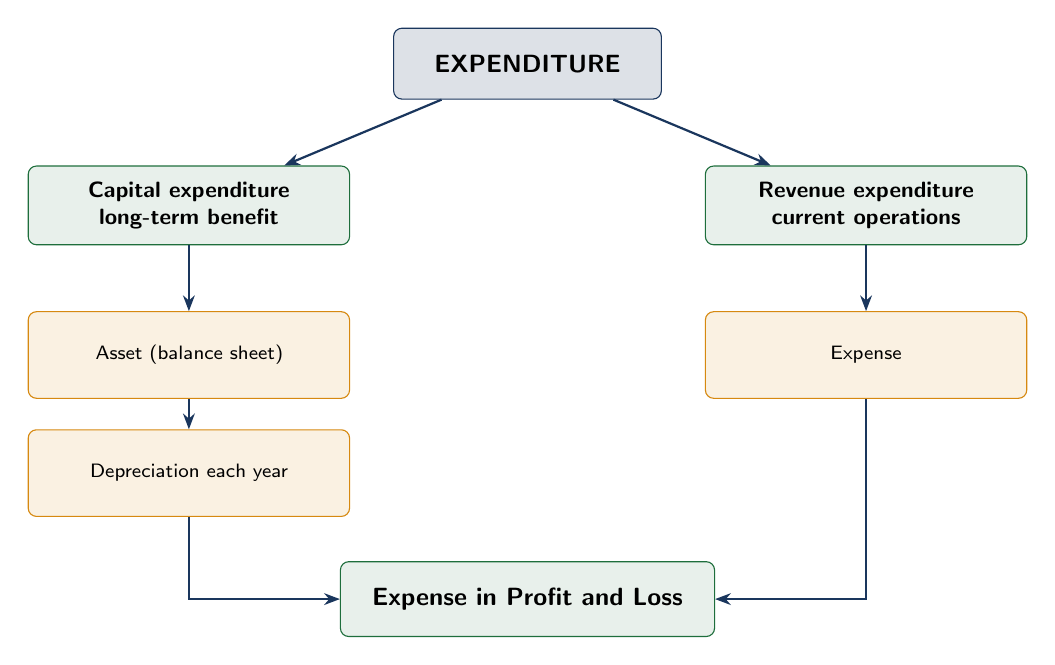
\begin{tikzpicture}[node distance=0.5cm]
  \node[lvl0,minimum width=3.4cm] (e) at (0,0) {EXPENDITURE};
  \node[lvl1,text width=3.8cm] (c) at (-4.3,-1.8) {Capital expenditure\\long-term benefit};
  \node[lvl1,text width=3.8cm] (r) at (4.3,-1.8) {Revenue expenditure\\current operations};
  \node[lvl2,text width=3.8cm] (a) at (-4.3,-3.7) {Asset (balance sheet)};
  \node[lvl2,text width=3.8cm] (d) at (-4.3,-5.2) {Depreciation each year};
  \node[lvl2,text width=3.8cm] (x) at (4.3,-3.7) {Expense};
  \node[outbox,text width=4.4cm] (p) at (0,-6.8) {Expense in Profit and Loss};
  \draw[arr] (e) -- (c); \draw[arr] (e) -- (r);
  \draw[arr] (c) -- (a); \draw[arr] (a) -- (d);
  \draw[arr] (r) -- (x);
  \draw[arr] (d) |- (p); \draw[arr] (x) |- (p);
\end{tikzpicture}
\end{center}

% =====================================================================
\section{Prepaid and Outstanding Expenses}

\subsection{Prepaid expense}

\begin{defbox}{Prepaid expense}
An amount \textbf{paid in advance} for a benefit that will be received in a \textbf{future period}.
\end{defbox}

\begin{exbox}{Insurance paid in advance}
Annual insurance of \Rs 1,20,000 is paid in advance. If \Rs 30,000 relates to the next accounting year, that
\Rs 30,000 is a \textbf{prepaid expense} at the reporting date. The expense of the current year is only the portion
relating to the current period:
\[
\text{Current-year expense}=1{,}20{,}000-30{,}000=\Rs\,90{,}000,\qquad\text{Prepaid}=\Rs\,30{,}000 .
\]
\end{exbox}

\[
\boxed{\text{Payment made now}\neq\text{Entire amount is current expense}}
\]

The unused portion is a future economic benefit and is treated separately (as an asset / prepayment).

\begin{center}
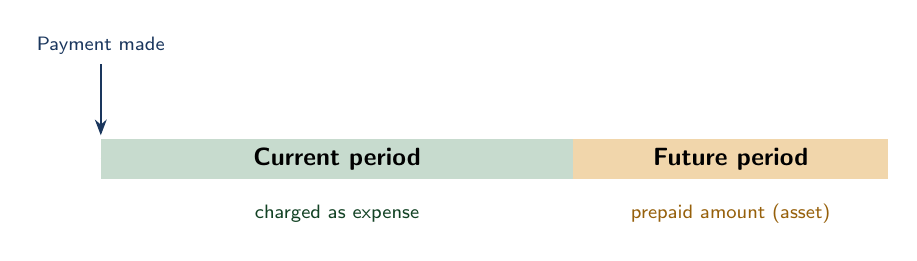
\begin{tikzpicture}
  \draw[thick,acnavy] (0,0) -- (10,0);
  \fill[acgreen!25] (0,-0.25) rectangle (6,0.25);
  \fill[acamber!35] (6,-0.25) rectangle (10,0.25);
  \node[font=\sffamily\small\bfseries] at (3,0) {Current period};
  \node[font=\sffamily\small\bfseries] at (8,0) {Future period};
  \draw[arr] (0,1.2) node[above,font=\sffamily\scriptsize] {Payment made} -- (0,0.3);
  \node[font=\sffamily\scriptsize,text=acgreen!60!black] at (3,-0.7) {charged as expense};
  \node[font=\sffamily\scriptsize,text=acamber!70!black] at (8,-0.7) {prepaid amount (asset)};
\end{tikzpicture}
\end{center}

\subsection{Outstanding expense}

\begin{defbox}{Outstanding expense}
An expense that (i) relates to the \textbf{current accounting period}, (ii) whose benefit has already been
\textbf{received or consumed}, but (iii) which has \textbf{not yet been paid}.
\end{defbox}

\begin{exbox}{Unpaid March salary}
Salary of \Rs 50,000 for March is still unpaid at year-end. The employees have already provided the service, so
the salary is an expense of the current period. Payment has not been made, so it is also an obligation.
It is recognised as an \textbf{expense} in the Income Statement and a \textbf{liability} in the Balance Sheet.
\end{exbox}

\[
\boxed{\text{Outstanding expense}=\text{Expense incurred but not yet paid}}
\]

\subsection{Prepaid versus outstanding}

\begin{center}
\small
\begin{tabularx}{\textwidth}{@{}l Y Y@{}}
\toprule
\rowcolor{acnavy!15}\textbf{Basis} & \textbf{Prepaid expense} & \textbf{Outstanding expense}\\
\midrule
Payment & Already paid & Not yet paid\\
Benefit & Relates partly or fully to a future period & Already received or consumed\\
Current expense & Only the applicable current portion & The current-period amount is the expense\\
Balance sheet effect & \textbf{Asset} (prepayment) & \textbf{Liability}\\
Example & Insurance paid in advance & Salary due but unpaid\\
\bottomrule
\end{tabularx}
\end{center}

\begin{keybox}
\textbf{Prepaid: paid first, benefit later.} \quad \textbf{Outstanding: benefit first, payment later.}
\end{keybox}

% =====================================================================
\section{Income, Revenue, Profit, Gain and Loss}

\subsection{Income}

The lecture defines \textbf{income} as the profit earned during a period:
\[
\boxed{\text{Income}=\text{Revenue}-\text{Expense}}
\]

\begin{impbox}[Wider meaning of income]
In formal accounting terminology \textbf{income is broader than profit}: it can include revenue as well as gains,
depending on the framework. For this introductory treatment the working relationship is
$\text{Profit}=\text{Revenue}-\text{Expenses}$.
\end{impbox}

\subsection{Revenue}

\begin{defbox}{Revenue}
Income arising from the entity's \textbf{ordinary activities}, such as the sale of goods and the rendering
of services.
\end{defbox}

\begin{exbox}{Furniture sales}
A furniture business sells furniture worth \Rs 5,00,000. This \Rs 5 lakh, generated by its ordinary sales activity,
is \textbf{revenue}.
\end{exbox}

\subsection{Profit}

\begin{defbox}{Profit}
The excess of revenue over the related costs / expenses.
\end{defbox}

\[
\boxed{\text{Profit}=\text{Revenue}-\text{Expenses}}
\]

\begin{exbox}{Profit}
Revenue \Rs 8,00,000, expenses \Rs 6,00,000: $\text{Profit}=8{,}00{,}000-6{,}00{,}000=\Rs\,2{,}00{,}000$.
Profit generally \textbf{increases the owner's equity}.
\end{exbox}

\subsection{Gain}

\begin{defbox}{Gain}
A profit arising from an activity that is generally \textbf{incidental, irregular or non-recurring}, rather than
from the ordinary sale of goods or services.
\end{defbox}

\begin{exbox}{Gain on sale of a machine}
A machine with a carrying / cost amount of \Rs 25,000 is sold for \Rs 28,000. $\text{Gain}=28{,}000-25{,}000=\Rs\,3{,}000$.
The business's ordinary activity is manufacturing or selling furniture, not selling machinery, so the \Rs 3,000 is a
\textbf{gain}, not ordinary sales revenue.
\end{exbox}

\subsection{Loss}

\begin{defbox}{Loss}
Arises when expenses or costs exceed the related revenue, or when an adverse event causes a reduction in economic
benefits. (Lecture: an excess of expenses over related revenues.)
\end{defbox}

\begin{exbox}{Loss}
Revenue \Rs 4,00,000, expenses \Rs 4,80,000: $\text{Loss}=4{,}80{,}000-4{,}00{,}000=\Rs\,80{,}000$.
A loss \textbf{decreases the owner's equity}.
\end{exbox}

\subsection{Revenue versus gain}

\begin{center}
\small
\begin{tabularx}{\textwidth}{@{}Y Y@{}}
\toprule
\rowcolor{acnavy!15}\textbf{Revenue} & \textbf{Gain}\\
\midrule
Arises from ordinary activities & Usually arises from incidental or non-core activities\\
Recurring in many businesses & Often irregular or non-recurring\\
Example: sale of goods by a trading company & Example: profit on sale of machinery\\
Part of ordinary operating income & Arises outside normal revenue-generating activity\\
\bottomrule
\end{tabularx}
\end{center}

For a furniture business: selling furniture is \textbf{revenue}; selling an old machine above its carrying amount is a
\textbf{gain}.

\subsection{Profit versus gain}

\textbf{Profit} is the broader result of operations; a \textbf{gain} is an increase in economic benefit from an
incidental, non-core event. A gain can be \textbf{one component of overall profit}; they are not competing concepts:

\[
\text{Operating Revenue}-\text{Operating Expenses}+\text{Gain}-\text{Loss}=\text{Overall Profit}
\]
(subject to the accounting framework and other income / expense items).

\subsection{Loss versus expense}

\begin{center}
\small
\begin{tabularx}{\textwidth}{@{}l Y Y@{}}
\toprule
\rowcolor{acnavy!15} & \textbf{Expense} & \textbf{Loss}\\
\midrule
\textbf{Nature} & Consumption of resources in carrying out \emph{normal} business activities & An \emph{unfavourable outcome}, often from an incidental event, or expenses exceeding related income\\
\textbf{Examples} & Salary, rent, electricity & Loss due to theft; loss on sale of machinery; loss from damage in an unexpected event\\
\textbf{One-liner} & Cost of earning revenue & Unfavourable economic outcome\\
\bottomrule
\end{tabularx}
\end{center}

\begin{center}
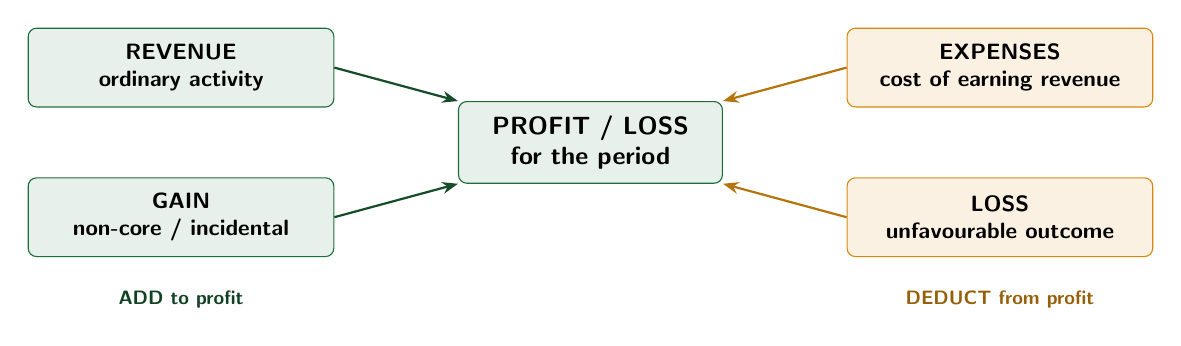
\begin{tikzpicture}
  \node[lvl1,text width=3.6cm] (rev) at (-5.2,0.95) {REVENUE\\ordinary activity};
  \node[lvl1,text width=3.6cm] (gain) at (-5.2,-0.95) {GAIN\\non-core / incidental};
  \node[lvl1,text width=3.6cm,draw=acamber,fill=acamber!12] (exp) at (5.2,0.95) {EXPENSES\\cost of earning revenue};
  \node[lvl1,text width=3.6cm,draw=acamber,fill=acamber!12] (loss) at (5.2,-0.95) {LOSS\\unfavourable outcome};
  \node[outbox,text width=3.0cm] (res) at (0,0) {PROFIT / LOSS\\for the period};
  \draw[arr,acgreen!70!black] (rev.east) -- (res.north west);
  \draw[arr,acgreen!70!black] (gain.east) -- (res.south west);
  \draw[arr,acamber!85!black] (exp.west) -- (res.north east);
  \draw[arr,acamber!85!black] (loss.west) -- (res.south east);
  \node[font=\sffamily\scriptsize\bfseries,text=acgreen!60!black] at (-5.2,-2.0) {ADD to profit};
  \node[font=\sffamily\scriptsize\bfseries,text=acamber!70!black] at (5.2,-2.0) {DEDUCT from profit};
\end{tikzpicture}
\end{center}

\subsection{Case study: identifying the terms (furniture business)}

\begin{casebox}{Which term applies?}
\begin{center}
\small
\begin{tabularx}{\textwidth}{@{}Y l Y@{}}
\toprule
\rowcolor{acteal!15}\textbf{Transaction / event} & \textbf{Term} & \textbf{Reason}\\
\midrule
Sold goods worth \Rs 50,000 to Mr.\ X & Sales / Revenue & Ordinary sale of business goods\\
Theft of cash from the office & Loss & Unfavourable reduction in resources\\
Sold goods costing \Rs 10,000 for \Rs 12,000 & Revenue $+$ Profit & \Rs 12,000 sales revenue; \Rs 2,000 gross profit before other costs\\
Machinery costing \Rs 25,000 sold for \Rs 28,000 & Gain & \Rs 3,000 gain on disposal of a non-current asset\\
\bottomrule
\end{tabularx}
\end{center}
\textbf{Calculations.} Goods: sales \Rs 12,000 $-$ cost \Rs 10,000 $=$ \textbf{profit \Rs 2,000}.
Machinery: proceeds \Rs 28,000 $-$ cost / carrying amount \Rs 25,000 $=$ \textbf{gain \Rs 3,000}.
\end{casebox}

% =====================================================================
\section{Terms Related to Trade}

This section introduces the vocabulary used for buying and selling goods.

\subsection{Purchases}

\begin{defbox}{Purchases}
Buying goods in which the business \textbf{ordinarily deals}, for the purpose of \textbf{resale}.
\end{defbox}

A furniture trader who buys furniture worth \Rs 1,00,000 for resale has \textbf{Purchases $=\Rs\,1{,}00{,}000$}.

\begin{impbox}[Purchase of goods vs.\ purchase of an asset]
If the furniture trader buys a \emph{computer for office use}, that is generally \textbf{not} a purchase of goods for
the trading account; it is the \textbf{acquisition of an asset}. ``Purchase'' in the accounting sense often means
specifically \emph{goods bought for resale}.
\end{impbox}

\subsection{Purchase return (returns outward)}

When goods previously purchased are \textbf{returned by the business to its supplier}, the return is called
\textbf{Purchase Return} or \textbf{Returns Outward}.

\begin{exbox}{Defective goods returned}
Goods worth \Rs 10,000 were purchased; defective goods worth \Rs 2,000 are returned. Purchase Returns $=\Rs\,2{,}000$.
\[
\boxed{\text{Net Purchases}=\text{Purchases}-\text{Purchase Returns}}\quad\Rightarrow\quad 10{,}000-2{,}000=\Rs\,8{,}000
\]
\end{exbox}

\subsection{Sales}

\begin{defbox}{Sales}
The transfer / sale of goods or services to customers for consideration. For a trading business, the sale of goods
in which it deals.
\end{defbox}

A furniture trader sells goods worth \Rs 50,000, so \textbf{Sales $=\Rs\,50{,}000$}. Sales are a major source of
\textbf{revenue} for a trading business.

\subsection{Sales return (returns inward)}

When customers \textbf{return goods} previously sold by the business, it is called \textbf{Sales Return} or
\textbf{Returns Inward}.

\begin{exbox}{Customer returns goods}
Goods sold for \Rs 20,000; the customer returns goods worth \Rs 3,000. Sales Returns $=\Rs\,3{,}000$.
\[
\boxed{\text{Net Sales}=\text{Sales}-\text{Sales Returns}}\quad\Rightarrow\quad 20{,}000-3{,}000=\Rs\,17{,}000
\]
\end{exbox}

\textbf{Memory trick.} \textbf{Returns Outward} $\rightarrow$ Purchase Return: the goods go \emph{out of} the
business, back to the supplier. \textbf{Returns Inward} $\rightarrow$ Sales Return: the goods come \emph{in to} the
business from the customer.

\subsection{Purchases versus sales}

\begin{center}
\small
\begin{tabularx}{\textwidth}{@{}l Y@{}}
\toprule
\rowcolor{acnavy!15}\textbf{Term} & \textbf{Meaning}\\
\midrule
\textbf{Purchases} & Goods bought for resale\\
\textbf{Purchase return / returns outward} & Goods returned to the supplier\\
\textbf{Sales} & Goods sold to customers\\
\textbf{Sales return / returns inward} & Goods returned by customers\\
\bottomrule
\end{tabularx}
\end{center}

\begin{center}
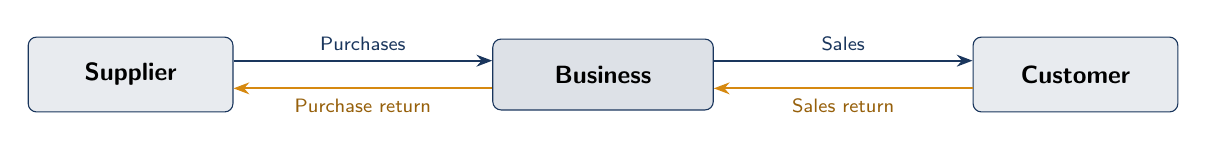
\begin{tikzpicture}
  \node[flowbox,minimum width=2.6cm] (s) at (0,0) {Supplier};
  \node[lvl0,minimum width=2.8cm] (b) at (6.0,0) {Business};
  \node[flowbox,minimum width=2.6cm] (c) at (12.0,0) {Customer};
  \draw[arr] ([yshift=5pt]s.east) -- node[above,font=\sffamily\scriptsize]{Purchases} ([yshift=5pt]b.west);
  \draw[arr,acamber] ([yshift=-5pt]b.west) -- node[below,font=\sffamily\scriptsize,text=acamber!70!black]{Purchase return} ([yshift=-5pt]s.east);
  \draw[arr] ([yshift=5pt]b.east) -- node[above,font=\sffamily\scriptsize]{Sales} ([yshift=5pt]c.west);
  \draw[arr,acamber] ([yshift=-5pt]c.west) -- node[below,font=\sffamily\scriptsize,text=acamber!70!black]{Sales return} ([yshift=-5pt]b.east);
\end{tikzpicture}
\end{center}

% =====================================================================
\section{Stock and Inventory}

\subsection{Stock}

\begin{defbox}{Stock}
Goods purchased for resale that \textbf{remain unsold} at the end of the accounting period.
\end{defbox}

\begin{exbox}{Closing stock}
A trader purchases goods worth \Rs 5,00,000. By year-end goods sold $=\Rs\,4{,}00{,}000$ and goods remaining
$=\Rs\,1{,}00{,}000$. The \textbf{closing stock is \Rs 1,00,000}, subject to the applicable inventory measurement
rules.
\end{exbox}

\subsection{Inventory}

\textbf{Inventory} is a \textbf{broader term} than stock in the lecture's traditional terminology. It can include:

\begin{center}
\small
\begin{tabularx}{\textwidth}{@{}l Y Y@{}}
\toprule
\rowcolor{acnavy!15}\textbf{Component} & \textbf{Meaning} & \textbf{Furniture example}\\
\midrule
\textbf{Raw materials} & Materials that will be used in production & Wood, nails, glue, other production materials\\
\textbf{Semi-finished goods / WIP} & Goods that have entered production but are not yet finished & A partially assembled table at year-end\\
\textbf{Finished goods} & Goods that have completed production and are held for sale & Completed tables awaiting sale\\
\textbf{Stock} & In the lecture's traditional trading terminology, finished / trading goods held for resale and unsold & Furniture held for resale\\
\bottomrule
\end{tabularx}
\end{center}

\[
\boxed{\text{Inventory}\supset\text{Stock}}\quad\text{(in the lecture's terminology)}
\]

\subsection{Stock versus inventory}

\begin{center}
\small
\begin{tabularx}{\textwidth}{@{}Y Y@{}}
\toprule
\rowcolor{acnavy!15}\textbf{Stock} & \textbf{Inventory}\\
\midrule
Narrower term in the lecture & Broader term\\
Mainly goods held for resale & Includes raw materials, WIP, finished goods and stock\\
Particularly relevant to trading goods & Also useful for manufacturing businesses\\
\bottomrule
\end{tabularx}
\end{center}

For a furniture manufacturer:
\[
\text{Raw materials}+\text{WIP}+\text{Finished goods}=\text{Inventory},
\]
and the finished goods held for sale may be called \textbf{stock} in the traditional terminology.

% =====================================================================
\section{Bills Receivable and Bills Payable}

\subsection{Bills receivable}

\begin{defbox}{Bill receivable}
A \textbf{bill of exchange} drawn on a debtor, or received by the business by endorsement from another party, under
which the specified amount is \textbf{receivable at a future date}.
\end{defbox}

In simple terms: a formal written right to receive money in the future.

\begin{exbox}{Customer accepts a bill}
A customer owes \Rs 50,000. Instead of an informal credit balance, the customer accepts a bill promising to pay
\Rs 50,000 after 3 months. For the business, \textbf{Bill Receivable $=\Rs\,50{,}000$}: an amount it expects to
\emph{receive} in the future.
\end{exbox}

\subsection{Bills payable}

\begin{defbox}{Bill payable}
A bill of exchange \textbf{accepted by the business in favour of a creditor}, under which the business must
\textbf{pay} the specified amount at a future date.
\end{defbox}

\begin{exbox}{Business accepts a bill}
The business owes a supplier \Rs 60,000 and accepts a bill payable after three months.
\textbf{Bill Payable $=\Rs\,60{,}000$}, a \textbf{liability}.
\end{exbox}

\subsection{Bills receivable versus bills payable}

\begin{center}
\small
\begin{tabularx}{\textwidth}{@{}Y Y@{}}
\toprule
\rowcolor{acnavy!15}\textbf{Bills receivable} & \textbf{Bills payable}\\
\midrule
Amount to be \textbf{received} & Amount to be \textbf{paid}\\
Asset in the usual classification & Liability in the usual classification\\
Usually arises from debtors & Usually arises from creditors\\
Gives a right to receive money & Creates an obligation to pay money\\
Future inflow & Future outflow\\
\bottomrule
\end{tabularx}
\end{center}

\textbf{Memory trick.} \textbf{Receivable $=$ Receive}; \textbf{Payable $=$ Pay}.

% =====================================================================
\section{Debtors and Creditors}

\subsection{Debtors}

\begin{defbox}{Debtors}
Persons or firms to whom the business has sold goods or provided services \textbf{on credit} and from whom payment
has not yet been received.
\end{defbox}

\textbf{Debtors owe money to the business.} If a business sells goods worth \Rs 1,00,000 to X on credit, then until
X pays, X is a debtor. The amount is generally shown as a \textbf{trade receivable}.

\subsection{Creditors}

\begin{defbox}{Creditors}
Persons or firms from whom the business has purchased goods or obtained services \textbf{on credit} and to whom
payment is still due.
\end{defbox}

\textbf{Creditors are owed money by the business.} If a business purchases goods worth \Rs 80,000 from Y on credit,
then until it pays, Y is a creditor. The amount is generally a \textbf{trade payable}.

\subsection{Debtor versus creditor}

This is one of the easiest places to get confused.

\begin{center}
\small
\begin{tabularx}{\textwidth}{@{}l Y Y@{}}
\toprule
\rowcolor{acnavy!15} & \textbf{Debtor} & \textbf{Creditor}\\
\midrule
\textbf{Meaning} & Someone who \textbf{owes us} money & Someone \textbf{whom we owe} money\\
\textbf{Balance sheet} & Receivable (asset) & Payable (liability)\\
\textbf{Memory} & Debtor $\rightarrow$ \emph{Due to us} & Creditor $\rightarrow$ \emph{Credit given to us}\\
\bottomrule
\end{tabularx}
\end{center}

\begin{exbox}{A, B and C}
\textbf{A sells \Rs 20,000 of goods on credit to B}: for A, \textbf{B is a debtor}.
\textbf{A buys \Rs 15,000 of goods on credit from C}: for A, \textbf{C is a creditor}.
\end{exbox}

\begin{impbox}[Viewpoint matters]
The same person can be a debtor in one set of books and a creditor in another. In the example above, B is a
debtor of A, but \emph{in B's own books} A is a creditor. Always ask: ``whose books am I looking at?''
\end{impbox}

% =====================================================================
\section{Bad Debts and Insolvency}

\subsection{Bad debts}

\begin{defbox}{Bad debt}
An amount due from a debtor that has become \textbf{irrecoverable}.
\end{defbox}

A customer owes \Rs 50,000 but becomes unable to pay and the amount is determined to be irrecoverable. Then
\textbf{Bad debt $=\Rs\,50{,}000$}. It is a \textbf{loss to the business}, and the lecture states that bad debts are
charged to the \textbf{Profit and Loss Account as an expense / loss}.

\textbf{Effect:}
\[
\text{Debtors / Receivables}\downarrow\quad\Rightarrow\quad\text{Profit}\downarrow\quad\Rightarrow\quad\text{Equity}\downarrow
\]

\begin{exbox}{Bad debt}
Debtors total \Rs 3,00,000. A debtor owing \Rs 20,000 becomes insolvent and the amount cannot be recovered.
\[
\text{Bad debt}=\Rs\,20{,}000,\qquad\text{Remaining receivables}=3{,}00{,}000-20{,}000=\Rs\,2{,}80{,}000 .
\]
The \Rs 20,000 is recognised as a loss / expense under the applicable accounting treatment.
\end{exbox}

\subsection{Insolvent / insolvency}

\begin{defbox}{Insolvent}
A person or enterprise that is not in a position to pay its debts. Depending on the legal framework, it may also
mean that liabilities exceed assets.
\end{defbox}

\textbf{Relationship to bad debt.} If Business A is owed money by Customer B and B becomes insolvent and cannot
repay, A may suffer a bad debt:

\[
\text{Insolvency of debtor}\;\rightarrow\;\text{Possible irrecoverability}\;\rightarrow\;\text{Bad debt for the creditor}
\]

% =====================================================================
\section{Discount}

A \textbf{discount} is a rebate or allowance given by the seller to the buyer. The lecture divides it into two types:

\[
\boxed{\text{Trade Discount}\quad+\quad\text{Cash Discount}}
\]

\subsection{Trade discount}

\begin{defbox}{Trade discount}
A discount given at a stated percentage on the \textbf{list / catalogue price} of goods, for commercial reasons
such as bulk purchases, dealer arrangements, regular trade relationships or wholesale pricing.
\end{defbox}

\begin{impbox}[Accounting treatment]
\textbf{Trade discount is not recorded separately in the books of account.} It is deducted from the list price when
determining the invoice amount, and the transaction is recorded at the net amount.
\end{impbox}

\begin{exbox}{Trade discount}
List price \Rs 1,00,000; trade discount 10\%.
\[
\text{Discount}=1{,}00{,}000\times10\%=\Rs\,10{,}000,\qquad \text{Invoice value}=1{,}00{,}000-10{,}000=\Rs\,90{,}000 .
\]
The transaction is recorded at \textbf{\Rs 90,000}, not as a \Rs 1,00,000 purchase plus a separate \Rs 10,000 discount.
\end{exbox}

\subsection{Cash discount}

\begin{defbox}{Cash discount}
An allowance given for \textbf{prompt or early payment}. Unlike trade discount, \textbf{cash discount is recorded in
the books}.
\end{defbox}

\begin{exbox}{Cash discount}
Amount due \Rs 50,000; cash discount for prompt payment 5\%.
\[
\text{Discount}=50{,}000\times5\%=\Rs\,2{,}500,\qquad\text{Cash paid}=50{,}000-2{,}500=\Rs\,47{,}500 .
\]
For the \textbf{seller} this is \emph{Discount Allowed}; for the \textbf{buyer} it is \emph{Discount Received}.
\end{exbox}

\subsection{Trade discount versus cash discount}

\begin{center}
\small
\begin{tabularx}{\textwidth}{@{}l Y Y@{}}
\toprule
\rowcolor{acnavy!15}\textbf{Basis} & \textbf{Trade discount} & \textbf{Cash discount}\\
\midrule
\textbf{Purpose} & Commercial / quantity / dealer discount & Prompt payment\\
\textbf{When given} & Usually at the time of sale or invoicing & At the time of settlement or payment\\
\textbf{Recorded separately?} & Generally \textbf{No} & \textbf{Yes}\\
\textbf{Shown in invoice?} & Usually deducted from list price & Usually depends on payment terms and settlement\\
\textbf{Example} & 10\% wholesale discount & 5\% discount for paying within 10 days\\
\bottomrule
\end{tabularx}
\end{center}

\textbf{Memory trick.} Trade discount $=$ \emph{discount on price}. Cash discount $=$ \emph{discount on payment}.

% =====================================================================
\section{A Comprehensive Example Combining the Terms}

\begin{casebox}{From catalogue price to cash paid}
A furniture business receives a catalogue price of \Rs 1,00,000 from a supplier.

\begin{center}
\small
\begin{tabularx}{\textwidth}{@{}c Y r Y@{}}
\toprule
\rowcolor{acteal!15}\textbf{Step} & \textbf{What happens} & \textbf{Amount (\Rs)} & \textbf{Term}\\
\midrule
1 & Supplier gives a 10\% trade discount: $1{,}00{,}000-10{,}000$ & 90,000 invoice & Trade discount (not separately recorded)\\
2 & Furniture bought on credit & 90,000 & Purchases; Creditor\\
3 & Furniture worth \Rs 10,000 returned & 10,000 & Purchase return\\
4 & Remaining payable: $90{,}000-10{,}000$ & 80,000 & Creditor\\
5 & 5\% cash discount for immediate settlement: $80{,}000\times5\%$ & 4,000 & Cash discount (Discount Received)\\
6 & Cash paid: $80{,}000-4{,}000$ & 76,000 & Settlement\\
\bottomrule
\end{tabularx}
\end{center}
One example links:
\[
\text{Trade Discount}\rightarrow\text{Purchases}\rightarrow\text{Purchase Return}\rightarrow\text{Creditor}\rightarrow\text{Cash Discount}
\]
\end{casebox}

% =====================================================================
\section{Part II Reference Section}

\subsection{Comprehensive terminology table}

\begin{center}
\footnotesize
\begin{tabularx}{\textwidth}{@{}l Y l@{}}
\toprule
\rowcolor{acnavy!15}\textbf{Term} & \textbf{Meaning} & \textbf{Classification / effect}\\
\midrule
\textbf{Expenditure} & Incurrence of a cost through payment, transfer of property or liability for acquiring goods, assets or services & Broad term\\
\textbf{Capital expenditure} & Expenditure to acquire or improve long-term assets & Capitalised\\
\textbf{Revenue expenditure} & Expenditure for ordinary operations / maintenance & Generally expense\\
\textbf{Expense} & Cost whose benefit has been consumed or expired in the period & Reduces profit\\
\textbf{Prepaid expense} & Expense paid in advance for a future benefit & Asset / prepayment\\
\textbf{Outstanding expense} & Expense incurred but not yet paid & Liability\\
\textbf{Revenue} & Income from ordinary activities & Increases profit / equity\\
\textbf{Profit} & Excess of revenue over relevant expenses / costs & Increases equity\\
\textbf{Gain} & Profit from an incidental / non-core transaction & Increases profit / equity\\
\textbf{Loss} & Unfavourable outcome, or expenses exceeding related revenue & Reduces profit / equity\\
\textbf{Purchases} & Goods bought for resale & Trading item\\
\textbf{Purchase return} & Goods returned to supplier & Reduces purchases\\
\textbf{Sales} & Goods / services sold to customers & Revenue\\
\textbf{Sales return} & Goods returned by customers & Reduces sales\\
\textbf{Stock} & Unsold goods held for resale & Current asset / inventory\\
\textbf{Inventory} & Raw materials, WIP, finished goods and stock & Current asset\\
\textbf{Bills receivable} & Formal right to receive money under a bill & Asset\\
\textbf{Bills payable} & Formal obligation to pay under a bill & Liability\\
\textbf{Debtor} & Party owing money to the business & Receivable / asset\\
\textbf{Creditor} & Party to whom the business owes money & Payable / liability\\
\textbf{Bad debt} & Receivable that becomes irrecoverable & Loss / expense\\
\textbf{Insolvent} & Unable to meet debts / obligations & Financial / legal condition\\
\textbf{Trade discount} & Discount from list price, generally not separately recorded & Reduces invoice amount\\
\textbf{Cash discount} & Discount for prompt payment & Recorded separately\\
\bottomrule
\end{tabularx}
\end{center}

\subsection{High-value distinctions}

\begin{center}
\small
\begin{tabularx}{\textwidth}{@{}l Y Y@{}}
\toprule
\rowcolor{acnavy!15}\textbf{Pair} & \textbf{First term} & \textbf{Second term}\\
\midrule
Expenditure vs.\ expense & Expenditure $=$ cost \emph{incurred} & Expense $=$ cost \emph{consumed / expired}\\
Capital vs.\ revenue expenditure & Capital $\rightarrow$ long-term asset / future benefit & Revenue $\rightarrow$ current operations\\
Prepaid vs.\ outstanding & Prepaid $=$ paid now, benefit later & Outstanding $=$ benefit now, pay later\\
Revenue vs.\ gain & Revenue $=$ ordinary business activity & Gain $=$ incidental / non-core increase\\
Profit vs.\ gain & Profit $=$ overall result & Gain is \emph{one component} of overall profit\\
Expense vs.\ loss & Expense $=$ cost of resources consumed & Loss $=$ unfavourable economic outcome\\
Debtor vs.\ creditor & Debtor $=$ owes us & Creditor $=$ we owe them\\
Bills receivable vs.\ payable & Receivable $=$ receive later & Payable $=$ pay later\\
Trade vs.\ cash discount & Trade $=$ price discount; generally not recorded separately & Cash $=$ payment discount; recorded\\
\bottomrule
\end{tabularx}
\end{center}

\subsection{Important formulas and relationships}

\begin{center}
\small
\begin{tabularx}{\textwidth}{@{}l Y@{}}
\toprule
\rowcolor{acnavy!15}\textbf{Item} & \textbf{Formula}\\
\midrule
Profit & Revenue $-$ Expenses\\
Loss & Expenses $-$ Revenue (when expenses exceed revenue)\\
Net purchases & Purchases $-$ Purchase returns\\
Net sales & Sales $-$ Sales returns\\
Capital expenditure & $\rightarrow$ Asset $\rightarrow$ Depreciation / amortisation as applicable\\
Equity effect & Profit $\uparrow\Rightarrow$ Equity $\uparrow$; Loss $\uparrow\Rightarrow$ Equity $\downarrow$\\
\bottomrule
\end{tabularx}
\end{center}

\subsection{Master concept map for Part II}

\begin{center}
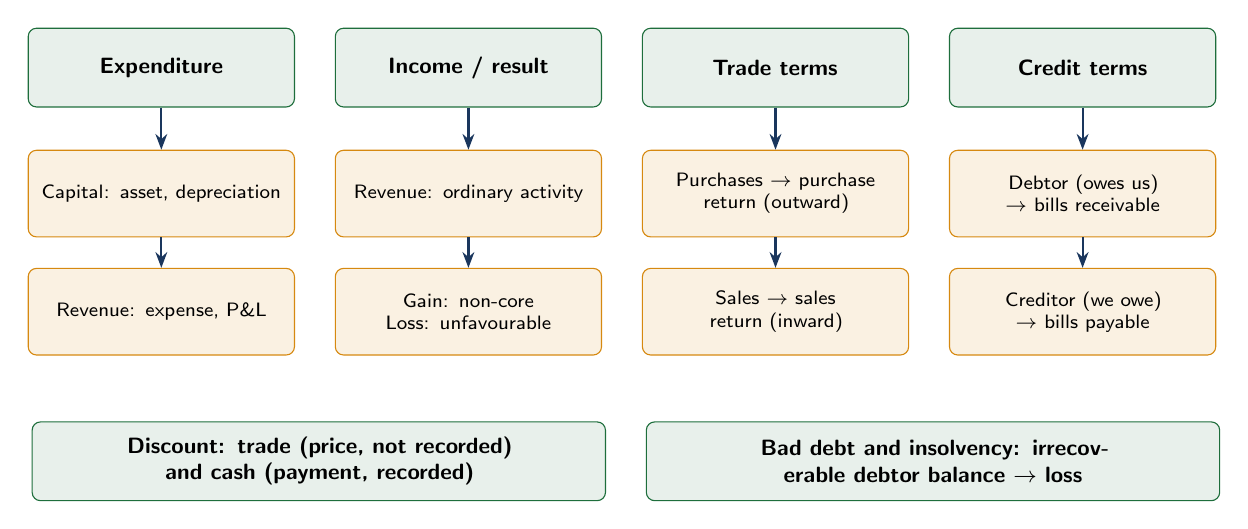
\begin{tikzpicture}
  \node[lvl1,text width=3.1cm] (exd) at (-5.9,0) {Expenditure};
  \node[lvl2,text width=3.1cm] (cx) at (-5.9,-1.6) {Capital: asset, depreciation};
  \node[lvl2,text width=3.1cm] (rx) at (-5.9,-3.1) {Revenue: expense, P\&L};
  \draw[arr] (exd) -- (cx); \draw[arr] (cx) -- (rx);
  \node[lvl1,text width=3.1cm] (inc) at (-2.0,0) {Income / result};
  \node[lvl2,text width=3.1cm] (i1) at (-2.0,-1.6) {Revenue: ordinary activity};
  \node[lvl2,text width=3.1cm] (i2) at (-2.0,-3.1) {Gain: non-core\\Loss: unfavourable};
  \draw[arr] (inc) -- (i1); \draw[arr] (i1) -- (i2);
  \node[lvl1,text width=3.1cm] (tr) at (1.9,0) {Trade terms};
  \node[lvl2,text width=3.1cm] (t1) at (1.9,-1.6) {Purchases $\to$ purchase return (outward)};
  \node[lvl2,text width=3.1cm] (t2) at (1.9,-3.1) {Sales $\to$ sales return (inward)};
  \draw[arr] (tr) -- (t1); \draw[arr] (t1) -- (t2);
  \node[lvl1,text width=3.1cm] (cr) at (5.8,0) {Credit terms};
  \node[lvl2,text width=3.1cm] (c1) at (5.8,-1.6) {Debtor (owes us) $\to$ bills receivable};
  \node[lvl2,text width=3.1cm] (c2) at (5.8,-3.1) {Creditor (we owe) $\to$ bills payable};
  \draw[arr] (cr) -- (c1); \draw[arr] (c1) -- (c2);
  \node[lvl1,text width=7.0cm,draw=acgreen] (ds) at (-3.9,-5.0) {Discount: trade (price, not recorded) and cash (payment, recorded)};
  \node[lvl1,text width=7.0cm,draw=acgreen] (bd) at (3.9,-5.0) {Bad debt and insolvency: irrecoverable debtor balance $\to$ loss};
\end{tikzpicture}
\end{center}

\subsection{Exam-focused final revision}

\begin{center}
\small
\begin{tabularx}{\textwidth}{@{}l Y@{}}
\toprule
\rowcolor{acnavy!15}\textbf{Term} & \textbf{Learn exactly}\\
\midrule
Expenditure & Amount spent or liability incurred to acquire assets, goods or services\\
Capital expenditure & Expenditure to acquire or substantially improve long-term assets, giving benefit over multiple periods\\
Revenue expenditure & Expenditure in the normal course of business, generally consumed in the current period\\
Expense & A cost whose benefit has been consumed or expired during the accounting period\\
Prepaid expense & Paid now, benefit received later\\
Outstanding expense & Benefit received now, payment made later\\
Revenue & Income generated from ordinary business activities\\
Profit & Excess of revenue over expenses\\
Gain & Profit from an incidental / non-core transaction, such as sale of a fixed asset above its carrying amount\\
Loss & An unfavourable economic outcome or excess of expenses over related revenue\\
Purchases / Purchase return & Goods bought for resale / goods returned to suppliers (returns outward)\\
Sales / Sales return & Goods sold to customers / goods returned by customers (returns inward)\\
Stock / Inventory & Unsold goods held for resale / broader category including raw materials, WIP, finished goods and stock\\
Debtor / Creditor & Owes money \emph{to us} / \emph{we owe} money to\\
Bills receivable / payable & Money to be received / paid in the future under a bill\\
Bad debt / Insolvent & Irrecoverable amount due from a debtor / unable to meet debts or obligations\\
Trade / Cash discount & Reduction from list price, generally not separately recorded / reduction for prompt payment, recorded\\
\bottomrule
\end{tabularx}
\end{center}

\begin{keybox}
\textbf{One-line memory framework.}
Expenditure $\rightarrow$ cost incurred $\cdot$ Expense $\rightarrow$ cost consumed $\cdot$ Revenue $\rightarrow$ ordinary income $\cdot$
Gain $\rightarrow$ incidental profit $\cdot$ Loss $\rightarrow$ unfavourable outcome $\cdot$ Debtor $\rightarrow$ owes us $\cdot$
Creditor $\rightarrow$ we owe them $\cdot$ Receivable $\rightarrow$ receive later $\cdot$ Payable $\rightarrow$ pay later $\cdot$
Trade discount $\rightarrow$ price $\cdot$ Cash discount $\rightarrow$ payment.
\end{keybox}

% =====================================================================
%                              PART III  (2_C)
% =====================================================================
\partheader{Part III \ (Lecture 2\_C)}{Accounting Principles, Concepts and Conventions}{The principles and assumptions that govern how transactions are recognised, measured, recorded and presented}

\section{Accounting Principles and GAAP}

Part III is one of the most important theoretical sections of the introductory module. It explains the
\textbf{principles and assumptions that govern the preparation of accounting records and financial statements}.
The broad sequence is:

\[
\boxed{\text{Accounting Principles}\rightarrow\text{Accounting Concepts}\rightarrow\text{Accounting Conventions}}
\]

These ideas explain \textbf{how transactions should be recognised, measured, recorded and presented} so that
accounting information is meaningful and comparable.

\subsection{Accounting principles}

Financial statements come from a very large volume of information about the economic activities of an enterprise.
That information is accumulated, analysed, recorded and reported, and this should be done according to established
\textbf{accounting principles}.

\[
\text{Accumulated}\rightarrow\text{Analysed}\rightarrow\text{Recorded}\rightarrow\text{Reported}
\]

\begin{defbox}{Accounting principles}
The \textbf{basic rules, concepts and guidelines} that provide the foundation for recording transactions and
preparing financial statements.
\end{defbox}

They give guidance on how transactions should be \textbf{recorded}, how financial information should be
\textbf{measured}, what information should be \textbf{disclosed}, how financial statements should be
\textbf{prepared}, and how information should be \textbf{presented} to users.

\subsection{Generally Accepted Accounting Principles (GAAP)}

\begin{defbox}{GAAP}
\textbf{G}enerally \textbf{A}ccepted \textbf{A}ccounting \textbf{P}rinciples: the accepted body of accounting
principles, standards and practices used within a particular jurisdiction. It provides a framework for detailed
accounting rules and reporting practices.
\end{defbox}

The lecture describes GAAP as encompassing three layers:

\begin{center}
\small
\begin{tabularx}{\textwidth}{@{}c l Y@{}}
\toprule
\rowcolor{acnavy!15}\textbf{\#} & \textbf{Layer} & \textbf{What it contains}\\
\midrule
1 & Basic accounting principles / guidelines & The concepts and conventions in this Part\\
2 & Accounting standards & Issued by the relevant accounting standard-setting body\\
3 & Industry-specific practices & Where required for unusual or specialised situations\\
\bottomrule
\end{tabularx}
\end{center}

\begin{impbox}[GAAP is not one worldwide rulebook]
Accounting frameworks \textbf{differ by jurisdiction}; countries may use different standards or adaptations of
international standards. Conceptually, GAAP is the generally accepted framework of accounting rules and practices
\emph{within a jurisdiction}.
\end{impbox}

\subsection{Why accounting principles are needed}

Without common principles, two businesses could record the same economic event in completely different ways,
making financial statements difficult to compare, understand, analyse, audit and use for decisions. Principles
therefore promote:

\begin{center}
\small
\begin{tabularx}{\textwidth}{@{}l Y@{}}
\toprule
\rowcolor{acnavy!15}\textbf{Benefit} & \textbf{Meaning}\\
\midrule
\textbf{Consistency} & Similar transactions are treated in similar ways\\
\textbf{Comparability} & Statements of different periods or entities can be meaningfully compared\\
\textbf{Reliability and credibility} & Users have a structured basis for understanding the information\\
\textbf{Proper presentation} & Statements follow an organised framework rather than arbitrary treatment\\
\bottomrule
\end{tabularx}
\end{center}

\subsection{Overview: concepts and conventions}

The principles in this lecture fall into two groups:

\begin{center}
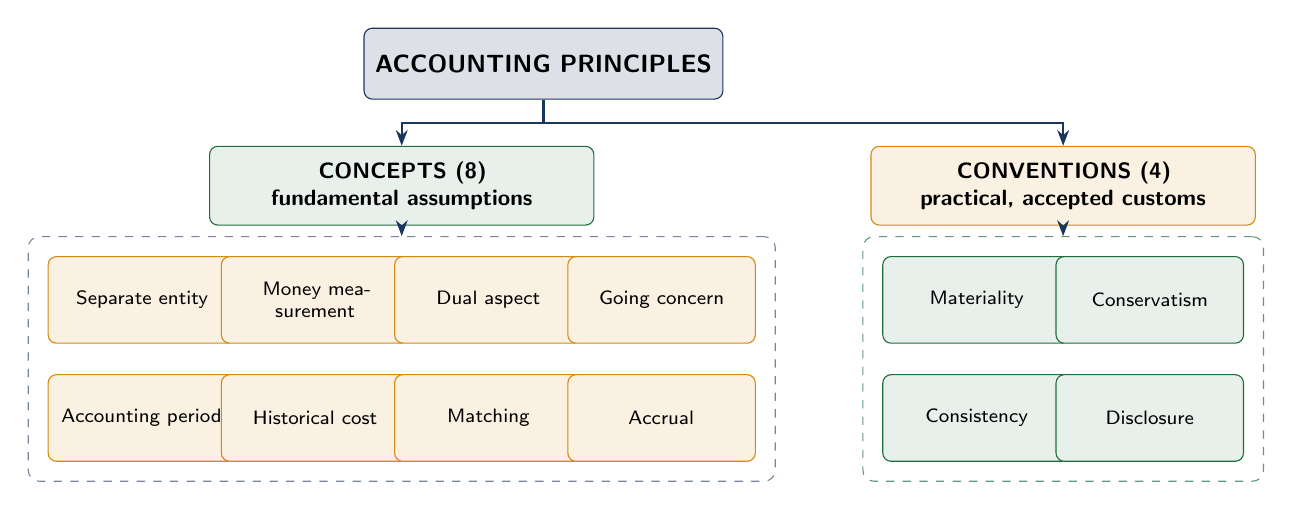
\begin{tikzpicture}
  \node[lvl0,minimum width=4.4cm] (root) at (-1.5,0) {ACCOUNTING PRINCIPLES};
  \node[lvl2,text width=2.1cm] (a1) at (-6.6,-3.0) {Separate entity};
  \node[lvl2,text width=2.1cm] (a2) at (-4.4,-3.0) {Money measurement};
  \node[lvl2,text width=2.1cm] (a3) at (-2.2,-3.0) {Dual aspect};
  \node[lvl2,text width=2.1cm] (a4) at (0.0,-3.0) {Going concern};
  \node[lvl2,text width=2.1cm] (b1) at (-6.6,-4.5) {Accounting period};
  \node[lvl2,text width=2.1cm] (b2) at (-4.4,-4.5) {Historical cost};
  \node[lvl2,text width=2.1cm] (b3) at (-2.2,-4.5) {Matching};
  \node[lvl2,text width=2.1cm] (b4) at (0.0,-4.5) {Accrual};
  \node[lvl2,text width=2.1cm,draw=acgreen,fill=acgreen!10] (c1) at (4.0,-3.0) {Materiality};
  \node[lvl2,text width=2.1cm,draw=acgreen,fill=acgreen!10] (c2) at (6.2,-3.0) {Conservatism};
  \node[lvl2,text width=2.1cm,draw=acgreen,fill=acgreen!10] (c3) at (4.0,-4.5) {Consistency};
  \node[lvl2,text width=2.1cm,draw=acgreen,fill=acgreen!10] (c4) at (6.2,-4.5) {Disclosure};
  \node[draw=acnavy!60,dashed,rounded corners=4pt,fit=(a1)(a4)(b1)(b4),inner sep=7pt,yshift=0pt] (g1) {};
  \node[draw=acgreen!70,dashed,rounded corners=4pt,fit=(c1)(c2)(c3)(c4),inner sep=7pt] (g2) {};
  \node[lvl1,text width=4.6cm] (con) at (-3.3,-1.55) {CONCEPTS (8)\\fundamental assumptions};
  \node[lvl1,text width=4.6cm,draw=acamber,fill=acamber!12] (conv) at (5.1,-1.55) {CONVENTIONS (4)\\practical, accepted customs};
  \draw[arr] (root.south) -- ++(0,-0.3) -| (con.north);
  \draw[arr] (root.south) -- ++(0,-0.3) -| (conv.north);
  \draw[arr] (con.south) -- (con.south |- g1.north);
  \draw[arr] (conv.south) -- (conv.south |- g2.north);
\end{tikzpicture}
\end{center}

% =====================================================================
\section{Accounting Concepts}

The eight accounting concepts are developed one by one below. Each follows the pattern: \emph{meaning},
\emph{example}, \emph{why it matters}.

% ---------------------------------------------------------------------
\subsection{Separate business entity concept}

\begin{defbox}{Separate business entity concept}
The \textbf{business and its owner are treated as separate entities} for accounting purposes. Even when a business
is owned by an individual, the accounting records are maintained from the \textbf{point of view of the business}.
\end{defbox}

\[
\boxed{\text{Business}\neq\text{Owner}}\quad\text{(for accounting purposes)}
\]

\begin{exbox}{Owner invests money}
The owner introduces \Rs 1,00,000 into the business. From the \emph{owner's} personal viewpoint, money has been given
to the business. From the \emph{business's} viewpoint, it has \textbf{received \Rs 1 lakh} and the owner's claim is
recorded as \textbf{Capital $=\Rs\,1{,}00{,}000$}. Cash rises; owner's equity (capital) rises.
\end{exbox}

\begin{exbox}{Owner withdraws money}
The owner withdraws \Rs 20,000 for personal use. The business records \textbf{Drawings $=\Rs\,20{,}000$}. It is
\emph{not} treated as a business expense merely because the business's cash has decreased. This is a direct
consequence of the separate-entity concept.
\end{exbox}

\textbf{Why it matters.} Without this separation it would be hard to determine how much belongs to the business and
how much to the owner, what the actual business expenses are, and what the business's real financial position is.

\begin{keybox}
Personal transactions of the owner should not be mixed with business transactions unless accounting principles
specifically require recognition. \emph{Question answered: whose transactions are we recording?}
\end{keybox}

% ---------------------------------------------------------------------
\subsection{Money measurement concept}

\begin{defbox}{Money measurement concept}
Accounting records only those transactions and events that can be \textbf{expressed in monetary terms}.
\end{defbox}

\[
\boxed{\text{Recordable accounting information}\Rightarrow\text{Measurable in money}}
\]

A fact may be important to the business and still not be recorded if it cannot be reliably expressed in money.

\begin{exbox}{Valuable but unrecorded}
A company has an exceptionally skilled management team. This may be very valuable, but the \emph{quality} of the team
is not ordinarily recorded as a monetary asset because it is hard to assign a sufficiently objective accounting value.
The lecture's other example: the \textbf{general health condition of a Managing Director} could affect the business,
but it is not normally an accounting transaction because it is not a monetary transaction.
\end{exbox}

\subsubsection{Limitations of the money measurement concept}

\textbf{1. Qualitative information may be excluded.} Facts that cannot be expressed reliably in money may not appear
in the records, for example employee morale, quality of management, reputation, industrial relations, health of key
personnel and customer loyalty.
\[
\boxed{\text{Financial statements do not capture every economically relevant fact}}
\]

\textbf{2. Assumption of a stable monetary unit.} Accounting generally assumes the monetary unit is a sufficiently
stable basis of measurement; the lecture states this as a \emph{stable or constant value of the rupee}. In reality
purchasing power changes through inflation, so \Rs 1 lakh today does not necessarily have the same purchasing power as
\Rs 1 lakh several years ago. This is one reason historical financial information needs careful interpretation.

\begin{keybox}
\emph{Question answered: which events can be recorded?}
\end{keybox}

% ---------------------------------------------------------------------
\subsection{Dual aspect concept}

\begin{defbox}{Dual aspect concept}
Every business transaction has \textbf{two accounting aspects (effects)}. This is the conceptual foundation of the
\textbf{double-entry bookkeeping system}.
\end{defbox}

\[
\boxed{\text{Every transaction has at least two effects}}
\]

These two effects keep the accounting equation balanced.

\begin{exbox}{Cash sale of \Rs 10,000}
\textbf{Aspect 1:} goods are transferred to the customer, so the business's inventory decreases.
\textbf{Aspect 2:} cash is received, so the business's cash increases.
One transaction, two effects.

\textbf{Equation view} (simplified): Cash $\uparrow$ and Sales / income $\uparrow$; since income ultimately affects equity,
Equity $\uparrow$. The accounting equation remains balanced.
\end{exbox}

\begin{exbox}{Furniture bought for cash, \Rs 50,000}
Furniture $\uparrow\Rs\,50{,}000$ and Cash $\downarrow\Rs\,50{,}000$. Total assets do not change
($+50{,}000-50{,}000=0$) but their \textbf{composition} does. This shows that ``dual aspect'' does not mean total
assets must always rise or fall; it means the transaction has \textbf{two corresponding effects}.
\end{exbox}

\subsubsection{Dual aspect and the accounting equation}

\[
\boxed{\text{Assets}=\text{Liabilities}+\text{Equity}}
\]
or, in the course's traditional terms,
\[
\boxed{\text{Assets}=\text{Liabilities}+\text{Capital}}
\]

Every transaction must affect the equation so that it remains balanced, which is why the concept is fundamental to
double-entry accounting.

\begin{keybox}
\emph{Question answered: how many effects does each transaction have?}
\end{keybox}

% ---------------------------------------------------------------------
\subsection{Going concern concept}

\begin{defbox}{Going concern concept}
The business is assumed to \textbf{continue its operations for the foreseeable future} rather than being forced to
liquidate in the immediate future, unless there is evidence to the contrary.
\end{defbox}

\subsubsection{Why the assumption is necessary}

A machine is bought for \Rs 10,00,000 and is expected to last 10 years. If the business is assumed to continue, it
makes sense to treat the machine as giving benefits over its useful life and to \textbf{allocate its cost through
depreciation}. If the business were about to shut down immediately, the relevant question would instead be: \emph{what
amount can actually be recovered by selling the machine?} So the assumption influences how assets and liabilities are
measured and presented.

\subsubsection{Implications of going concern}

\begin{itemize}
  \item Assets are generally \emph{not} treated as though they must all be sold immediately.
  \item Long-term assets can be used over their useful lives.
  \item Costs can be allocated across accounting periods.
  \item Depreciation can be charged over the useful life of assets.
  \item Long-term liabilities can be classified and presented according to their contractual terms.
\end{itemize}

\[
\boxed{\text{Going concern}\Rightarrow\text{Business is accounted for as an operating entity}}
\]
(rather than as an entity about to be liquidated).

\begin{keybox}
\emph{Question answered: what assumption do we make about the business's future?}
\end{keybox}

% ---------------------------------------------------------------------
\subsection{Accounting period concept}

A business may theoretically continue indefinitely, but users cannot wait indefinitely to learn its performance.
Therefore the life of a business is divided into \textbf{accounting periods}: a month, a quarter, six months or a
financial year. The \textbf{year} is the common reporting period.

\begin{defbox}{Accounting period concept}
The continuous life of a business is divided into defined \textbf{accounting periods} for measuring and reporting
financial performance.
\end{defbox}

\begin{exbox}{Why divide life into periods?}
A business starts in 2020 and continues until 2050. If accounts were prepared only in 2050, the owner would wait
30 years to learn the overall result. Instead accounts are prepared periodically
($2020\rightarrow2021\rightarrow2022\rightarrow\cdots$), which allows users to determine annual profit or loss, annual
expenses, the financial position at year-end and changes in performance over time.
\end{exbox}

\subsubsection{Financial year versus calendar year}

Businesses may use different reporting periods depending on prevailing practice, tradition, government requirements
and applicable regulations.

\begin{center}
\small
\begin{tabularx}{\textwidth}{@{}l Y@{}}
\toprule
\rowcolor{acnavy!15}\textbf{Period} & \textbf{Span}\\
\midrule
\textbf{Calendar year} & 1 January $\rightarrow$ 31 December\\
\textbf{Financial year} & A 12-month period that may differ from the calendar year, depending on jurisdiction and reporting requirements\\
\bottomrule
\end{tabularx}
\end{center}

\begin{keybox}
\emph{Question answered: when do we measure performance?}
\end{keybox}

% ---------------------------------------------------------------------
\subsection{Historical cost concept}

\begin{defbox}{Historical cost concept}
An asset is ordinarily \textbf{initially recorded at the cost incurred to acquire it}, rather than at its market value
on the purchase date.
\end{defbox}

\begin{exbox}{Plant bought for \Rs 5,00,000}
A business buys a plant for \Rs 5,00,000. At the time of purchase its market value happens to be \Rs 6,00,000.
Under the simplified historical-cost principle:
\[
\boxed{\text{Recorded cost}=\Rs\,5{,}00{,}000}
\]
because \Rs 5 lakh is the acquisition cost.
\end{exbox}

\subsubsection{Historical cost does not mean ``never changes''}

Historical cost does \textbf{not} mean an asset appears at exactly its original cost forever. Depreciable assets are
reduced through \textbf{depreciation}.

\begin{exbox}{Carrying amount after depreciation}
Original cost \Rs 5,00,000; cumulative depreciation \Rs 1,50,000.
\[
\text{Carrying amount}=5{,}00{,}000-1{,}50{,}000=\Rs\,3{,}50{,}000
\]
(subject to the relevant accounting rules). So
\[
\boxed{\text{Historical cost}\neq\text{Permanent unchanging book value}}
\]
\end{exbox}

\subsubsection{Why historical cost is useful}

\begin{itemize}
  \item It is based on an \textbf{actual transaction}.
  \item It is generally \textbf{easier to verify}.
  \item It provides \textbf{objective evidence} of the original acquisition amount.
  \item It reduces dependence on \textbf{subjective market estimates} at the acquisition date.
\end{itemize}

However, it can become \textbf{less representative of current economic value} as prices change (see the
limitation discussed in Part 1).

\begin{keybox}
\emph{Question answered: at what amount is an asset initially recorded?}
\end{keybox}

% ---------------------------------------------------------------------
\subsection{Matching concept}

\begin{defbox}{Matching concept}
Revenue earned during an accounting period must be \textbf{matched with the corresponding expenses} relating to that
revenue, so that the proper profit for the period can be determined.
\end{defbox}

\[
\boxed{\text{Profit}=\text{Revenue of period}-\text{Expenses relating to that revenue}}
\]

\begin{exbox}{Shop inventory}
A shop buys inventory for \Rs 1,00,000 during the year, but by year-end only goods costing \Rs 60,000 have been sold.
The full \Rs 1,00,000 should \emph{not} automatically be treated as the cost of the period's sales.
\begin{itemize}
  \item \Rs 60,000 is associated with goods \textbf{sold} (cost of sales);
  \item the remaining \Rs 40,000 relates to inventory \textbf{still held} and remains part of inventory, subject to
        the applicable inventory accounting rules.
\end{itemize}
\textbf{Central idea: match the cost with the revenue it helped generate.}
\end{exbox}

\begin{exbox}{Profit measurement}
Revenue \Rs 2,00,000; related expenses \Rs 1,20,000. $\text{Profit}=2{,}00{,}000-1{,}20{,}000=\textbf{\Rs 80{,}000}$.
The purpose of matching is to ensure reported profit is not distorted by assigning unrelated expenses to the period.
\end{exbox}

\begin{keybox}
\emph{Question answered: which costs belong with this period's revenue?}
\end{keybox}

% ---------------------------------------------------------------------
\subsection{Accrual concept}

\begin{defbox}{Accrual concept}
Transactions are recognised based on when \textbf{income is earned and expenses are incurred}, rather than when cash
is received or paid.
\end{defbox}

\[
\boxed{\text{Revenue}\rightarrow\text{when earned}}\qquad\boxed{\text{Expense}\rightarrow\text{when incurred}}
\]
not when cash is received or paid.

\begin{exbox}{Electricity}
The business uses electricity during March; the bill is received in March but paid in April. Under accrual
accounting the electricity expense belongs to \textbf{March}, because the service was consumed in March. Expense
recognition follows \emph{consumption / incurrence}, not the date of payment.
\end{exbox}

\subsubsection{Accrual versus cash basis}

\begin{center}
\small
\begin{tabularx}{\textwidth}{@{}Y Y@{}}
\toprule
\rowcolor{acnavy!15}\textbf{Accrual basis} & \textbf{Cash basis}\\
\midrule
Recognise revenue when earned & Recognise revenue when cash is received\\
Recognise expense when incurred & Recognise expense when cash is paid\\
Focuses on economic activity & Focuses on cash movement\\
Gives a fuller picture of period performance & Can differ substantially from economic performance\\
\bottomrule
\end{tabularx}
\end{center}

A customer buys goods on credit in March and pays in April. Under accrual accounting, revenue is recognised in
\textbf{March}, even though cash arrives in \textbf{April}.

\subsubsection{Relationship between matching and accrual}

\begin{center}
\small
\begin{tabularx}{\textwidth}{@{}l Y@{}}
\toprule
\rowcolor{acnavy!15}\textbf{Concept} & \textbf{Question it asks}\\
\midrule
\textbf{Accrual} & \emph{When} should the transaction's income or expense be recognised?\\
\textbf{Matching} & \emph{Which} expenses belong with the revenue of this period?\\
\bottomrule
\end{tabularx}
\end{center}

Together they give an economically meaningful measure of periodic profit.

\begin{keybox}
\emph{Question answered: when should income or expense be recognised?}
\end{keybox}

% =====================================================================
\section{Concepts versus Conventions}

\begin{center}
\small
\begin{tabularx}{\textwidth}{@{}Y Y@{}}
\toprule
\rowcolor{acnavy!15}\textbf{Accounting concepts} & \textbf{Accounting conventions}\\
\midrule
Fundamental assumptions / principles used in recording and reporting & Generally accepted customs or practices used as practical guides\\
Form the conceptual foundation & Help deal with practical reporting situations\\
More fundamental in nature & Often arise from accepted practice\\
Guide recognition, measurement and reporting & Guide consistent presentation and treatment\\
\bottomrule
\end{tabularx}
\end{center}

\[
\boxed{\text{Concept}=\text{Fundamental accounting idea / principle}}
\]
\[
\boxed{\text{Convention}=\text{Widely accepted practical practice}}
\]

% =====================================================================
\section{Accounting Conventions}

% ---------------------------------------------------------------------
\subsection{Materiality convention}

\begin{defbox}{Materiality convention}
Items of \textbf{small or insignificant importance} need not always receive the same detailed treatment that a highly
significant item would. Accounting procedures should be \textbf{proportionate to the importance of the item}.
\end{defbox}

\begin{exbox}{The \Rs 100 calculator}
An ordinary calculator costs \Rs 100 and could physically last 10 years. In theory its cost could be spread over
10 years. But the effort of classifying it as a long-term asset, calculating 10 years of depreciation and keeping
detailed records may exceed the benefit of such precision. Depending on the entity's accounting policy and
materiality threshold, it may simply be \textbf{treated as an expense of the period}.
\end{exbox}

\textbf{Materiality is relative.} An item can be material for one business and immaterial for another. \Rs 10,000 may
be insignificant for a large multinational but highly significant for a very small business.

\[
\boxed{\text{Materiality depends on context, size and significance}}
\]
It is a matter of \textbf{judgement}, not a universal fixed rupee amount.

\begin{keybox}
\emph{Question answered: does the item matter enough to warrant detailed treatment?}
\end{keybox}

% ---------------------------------------------------------------------
\subsection{Conservatism convention}

\begin{defbox}{Conservatism convention}
A \textbf{cautious} approach to accounting: anticipated expenses or losses should be recognised, while potential
income or gains should \textbf{not} be recognised prematurely.
\end{defbox}

\[
\boxed{\text{Do not overstate assets / profits}}\qquad\boxed{\text{Recognise probable losses appropriately}}
\]

\textbf{Example 1: doubtful debts.} A business has receivables and a reasonable expectation that some portion may not
be collected. Accounting may recognise an appropriate \textbf{allowance (provision) for doubtful receivables} rather
than assuming every amount will definitely be recovered.

\begin{exbox}{Example 2: inventory valuation (traditional rule)}
Value stock at \textbf{cost or market value, whichever is lower}. Cost \Rs 1,00,000; relevant market value \Rs 90,000.
Under the traditional lower-of-cost-or-market approach, \textbf{Value $=\Rs\,90{,}000$}. This avoids recognising an
unrealised increase but recognises a decline in value.
\end{exbox}

\begin{impbox}[Modern clarification]
Contemporary inventory accounting typically uses the \textbf{lower of cost and net realisable value (NRV)} rather
than the old broad ``cost or market'' formulation. The course uses the traditional example to illustrate
conservatism.
\end{impbox}

\textbf{Example 3: conservatism and gains.} A business owns an asset whose value has risen, but the increase has not
been realised or does not otherwise qualify for recognition. A conservative approach does not treat an uncertain,
unrealised increase as realised profit just because the asset \emph{could} be sold for more.
\[
\boxed{\text{Potential gain}\neq\text{Automatically recognised profit}}
\]
Recognition depends on the applicable accounting framework.

\begin{keybox}
\emph{Question answered: how should uncertainty be handled cautiously?}
\end{keybox}

% ---------------------------------------------------------------------
\subsection{Consistency convention}

\begin{defbox}{Consistency convention}
An entity should follow the \textbf{same accounting policies and methods for similar transactions over successive
periods}, unless there is a sound reason or an applicable requirement to change them. The objective is
\textbf{comparability over time}.
\end{defbox}

\begin{exbox}{Depreciation method}
A company chooses the \textbf{straight-line method} of depreciation for a class of assets. The method should
generally be applied consistently from year to year unless there is a justified reason to change, such as a change
required or permitted under the applicable framework. Changing arbitrarily every year would make comparison of
profits difficult.
\end{exbox}

\textbf{Why consistency matters.} Suppose Year 1 uses depreciation method A, Year 2 suddenly uses method B and Year 3
uses method C. Even if each is acceptable in some circumstances, switching without justification makes year-to-year
performance hard to compare.
\[
\boxed{\text{Consistency}\rightarrow\text{Comparability}}
\]

\begin{keybox}
\emph{Question answered: how do we maintain comparability across periods?}
\end{keybox}

% ---------------------------------------------------------------------
\subsection{Disclosure convention}

\begin{defbox}{Disclosure convention}
Financial statements should disclose the \textbf{material information} necessary for users to understand the
financial position and performance of the business and to make informed decisions.
\end{defbox}

Material information that could influence users' decisions should \textbf{not be concealed}.

\textbf{Why disclosure is important.} Financial statements contain summarised information, so users need enough
additional information to understand:

\begin{itemize}
  \item accounting policies,
  \item significant items,
  \item important uncertainties,
  \item major commitments,
  \item relevant risks,
  \item other material information.
\end{itemize}

\[
\boxed{\text{Financial statements}+\text{Required disclosures}\rightarrow\text{Useful information}}
\]

\begin{keybox}
\emph{Question answered: what information must users be told?}
\end{keybox}

% =====================================================================
\section{Master Tables and Relationships}

\subsection{The twelve at a glance}

\begin{center}
\small
\begin{tabularx}{\textwidth}{@{}l Y Y Y@{}}
\toprule
\rowcolor{acnavy!15}\textbf{Concept} & \textbf{Core idea} & \textbf{Simple example} & \textbf{Question it answers}\\
\midrule
\textbf{Separate entity} & Business and owner treated separately & Owner's investment recorded as capital & Whose transactions are we recording?\\
\textbf{Money measurement} & Only monetarily measurable information recorded & Employee morale not directly recorded & Which events can be recorded?\\
\textbf{Dual aspect} & Every transaction has two effects & Cash sale affects cash and sales & How many effects does each transaction have?\\
\textbf{Going concern} & Business assumed to continue operating & Machinery used over its useful life & What do we assume about the business's future?\\
\textbf{Accounting period} & Business life divided into reporting periods & Annual financial statements & When do we measure performance?\\
\textbf{Historical cost} & Asset initially recorded at acquisition cost & Plant bought for \Rs 5 lakh recorded at \Rs 5 lakh & At what amount is an asset initially recorded?\\
\textbf{Matching} & Match relevant expenses with related revenue & Cost of goods sold matched with sales & Which costs belong with this period's revenue?\\
\textbf{Accrual} & Recognise when earned / incurred & March electricity expense recognised in March & When should income / expense be recognised?\\
\midrule
\rowcolor{acamber!12}\textbf{Convention} & & &\\
\textbf{Materiality} & Insignificant items need not get disproportionate treatment & \Rs 100 calculator expensed & Does it matter enough for detailed treatment?\\
\textbf{Conservatism} & Avoid premature gains; recognise expected losses & Allowance for doubtful receivables & How do we handle uncertainty cautiously?\\
\textbf{Consistency} & Same methods for comparable transactions over time & Same depreciation method unless justified & How do we keep comparability across periods?\\
\textbf{Disclosure} & Material information adequately disclosed & Significant accounting policies & What must users be told?\\
\bottomrule
\end{tabularx}
\end{center}

\subsection{How the concepts work together}

\begin{center}
\small
\begin{tabularx}{\textwidth}{@{}l Y@{}}
\toprule
\rowcolor{acnavy!15}\textbf{Pair} & \textbf{Relationship}\\
\midrule
\textbf{Separate entity $+$ Dual aspect} & Separate entity decides \emph{whose books} we keep; dual aspect decides \emph{how transactions affect those books}\\
\textbf{Going concern $+$ Historical cost} & Because the business is assumed to continue, assets need not be valued as if sold immediately; historical cost can be the basis, followed by depreciation or other adjustments\\
\textbf{Accounting period $+$ Accrual} & The period tells us \emph{which period's performance} we measure; accrual tells us \emph{which revenues and expenses belong} to it\\
\textbf{Accrual $+$ Matching} & Accrual puts income and expenses in the right period; matching ensures the expenses linked to the revenue are charged to the same period $\rightarrow$ meaningful periodic profit\\
\textbf{Consistency $+$ Comparability} & Consistent methods $\rightarrow$ better comparison between periods\\
\textbf{Conservatism $+$ Disclosure} & Conservatism encourages cautious recognition and measurement; disclosure gives users the material information needed to understand the resulting figures\\
\bottomrule
\end{tabularx}
\end{center}

\subsection{Frequently confused concepts}

\begin{center}
\small
\begin{tabularx}{\textwidth}{@{}l Y Y@{}}
\toprule
\rowcolor{acnavy!15}\textbf{Pair} & \textbf{First asks} & \textbf{Second asks}\\
\midrule
Historical cost vs.\ matching & Historical cost: at what amount is an acquired asset \emph{initially recorded}? & Matching: which costs are recognised \emph{against revenue} in this period?\\
Accrual vs.\ matching & Accrual: \emph{when} to recognise? & Matching: \emph{which expense} belongs with which revenue / period?\\
Conservatism vs.\ historical cost & Historical cost sets the \emph{initial basis} of measurement & Conservatism deals with \emph{caution} when uncertainty exists\\
Consistency vs.\ disclosure & Consistency: use comparable methods \emph{over time} & Disclosure: give users the \emph{material information} they need\\
\bottomrule
\end{tabularx}
\end{center}

% =====================================================================
\section{A Complete Worked Example of the Concepts}

\begin{casebox}{One business, eight events}
\begin{enumerate}
  \item \textbf{Owner invests \Rs 10 lakh} (\emph{separate entity}). Recorded as capital of the business:
        Cash $\uparrow\Rs\,10{,}00{,}000$; Capital $\uparrow\Rs\,10{,}00{,}000$.
  \item \textbf{Business buys machinery for \Rs 4 lakh} (\emph{dual aspect}, \emph{historical cost}).
        Machinery $\uparrow\Rs\,4{,}00{,}000$; Cash $\downarrow\Rs\,4{,}00{,}000$. Machinery is initially recorded at its
        acquisition cost of \Rs 4,00,000.
  \item \textbf{Business purchases inventory for \Rs 2 lakh.} The inventory is initially recognised; the entire amount is
        \emph{not} immediately treated as a current-period expense. \emph{Matching} becomes relevant when it is sold.
  \item \textbf{Goods costing \Rs 80,000 are sold for \Rs 1,20,000} (\emph{matching}). Revenue \Rs 1,20,000, related cost
        \Rs 80,000, so $\text{Gross profit}=1{,}20{,}000-80{,}000=\textbf{\Rs 40{,}000}$.
  \item \textbf{Electricity of \Rs 10,000 relates to December but is paid in January} (\emph{accrual}). The expense belongs to
        \textbf{December}.
  \item \textbf{Some customer balances are doubtful} (\emph{conservatism}). An appropriate allowance for doubtful receivables
        may be recognised rather than assuming every receivable is certain to be collected.
  \item \textbf{Business uses straight-line depreciation} (\emph{consistency}). Apply the method consistently to similar assets
        unless a justified accounting reason requires a change.
  \item \textbf{Financial statements are prepared} (\emph{accounting period}, \emph{disclosure}). Transactions are assigned to the
        appropriate reporting period, and material information is properly disclosed.
\end{enumerate}
\medskip
This example shows the concepts operating \textbf{together}, not independently.
\end{casebox}

\subsection{A mental model: converting a business into financial statements}

\begin{center}
\small
\begin{tabularx}{\textwidth}{@{}c l Y@{}}
\toprule
\rowcolor{acnavy!15}\textbf{Step} & \textbf{Concept} & \textbf{Question to ask}\\
\midrule
1 & Separate entity & Whose transactions are we recording?\\
2 & Money measurement & Can the event be measured in monetary terms?\\
3 & Dual aspect & What are the two corresponding effects?\\
4 & Going concern & How should the business be viewed for accounting purposes?\\
5 & Accounting period & Which period are we reporting?\\
6 & Historical cost & At what amount is the asset initially recorded?\\
7 & Accrual & When was income earned or expense incurred?\\
8 & Matching & Which costs belong with this period's revenue?\\
9 & Materiality $+$ Conservatism $+$ Consistency $+$ Disclosure & How should information be presented sensibly, cautiously, consistently and transparently?\\
\bottomrule
\end{tabularx}
\end{center}

\subsection{Memory aids and exam definitions}

\textbf{Concepts (S--M--D--G--A--H--M--A):} \textbf{S}eparate Entity, \textbf{M}oney Measurement,
\textbf{D}ual Aspect, \textbf{G}oing Concern, \textbf{A}ccounting Period, \textbf{H}istorical Cost,
\textbf{M}atching, \textbf{A}ccrual.

\textbf{Conventions (M--C--C--D):} \textbf{M}ateriality, \textbf{C}onservatism, \textbf{C}onsistency, \textbf{D}isclosure.

\begin{center}
\small
\begin{tabularx}{\textwidth}{@{}l Y@{}}
\toprule
\rowcolor{acnavy!15}\textbf{Term} & \textbf{Exam definition}\\
\midrule
Separate business entity & The business is treated as a separate entity from its owner for accounting purposes, and transactions are recorded from the viewpoint of the business\\
Money measurement & Only transactions and events capable of being expressed in monetary terms are recognised in the accounting records\\
Dual aspect & Every business transaction has two accounting effects, forming the basis of the double-entry system\\
Going concern & The business is assumed to continue operating for the foreseeable future and is not expected to liquidate in the immediate future\\
Accounting period & The continuous life of a business is divided into appropriate accounting periods for measuring and reporting financial performance\\
Historical cost & Assets are initially recognised on the basis of the cost incurred to acquire them, subject to subsequent accounting adjustments\\
Matching & Revenue of an accounting period should be matched with the corresponding expenses incurred in earning that revenue to determine the proper profit for the period\\
Accrual & Revenue is recognised when earned and expenses when incurred, rather than merely when cash is received or paid\\
Materiality & Items that are insignificant in relation to the financial statements need not always receive disproportionately detailed accounting treatment\\
Conservatism & Accounting should avoid premature recognition of uncertain gains while appropriately recognising probable losses and obligations\\
Consistency & Accounting methods and policies should be applied consistently to similar transactions across periods unless a justified change is required or appropriate\\
Disclosure & Material information necessary for users to understand the financial statements and make informed decisions should be adequately disclosed\\
\bottomrule
\end{tabularx}
\end{center}

\subsection{One-page revision sheet}

\begin{center}
\small
\begin{tabularx}{\textwidth}{@{}l Y l Y@{}}
\toprule
\rowcolor{acnavy!15}\textbf{Concept} & \textbf{Keyword} & \textbf{Convention} & \textbf{Keyword}\\
\midrule
Separate entity & Business $\neq$ Owner & Materiality & Importance\\
Money measurement & Only monetary measurement & Conservatism & Caution\\
Dual aspect & Two effects & Consistency & Comparability\\
Going concern & Continue operating & Disclosure & Transparency\\
Accounting period & Divide time & & \\
Historical cost & Acquisition cost & & \\
Matching & Revenue $\leftrightarrow$ related cost & & \\
Accrual & Earned / incurred, not cash & & \\
\bottomrule
\end{tabularx}
\end{center}

\begin{keybox}
\textbf{Key equations of this Part:} $\text{Assets}=\text{Liabilities}+\text{Equity}$;\quad
$\text{Profit}=\text{Revenue}-\text{Expenses}$;\quad and conceptually
$\text{Accrual}+\text{Matching}\rightarrow\text{Proper periodic profit}$.
\end{keybox}

% =====================================================================
%                              PART IV
% =====================================================================
\partheader{Part IV}{Integrated Case Study and Revision}{All the terms, principles, concepts and conventions of Part 2 working together}

\section{Integrated Case Study: Meera Furniture Mart}

\begin{notebox}[About this case study]
This case study is \textbf{not in the lecture notes}. It was built for these notes to show the terms of Parts I and II
and the concepts of Part III operating together, using the same kinds of figures as the lecture examples.
\textbf{Assumptions:} the period is the business's \emph{first three months}; \textbf{depreciation and tax are ignored}
to keep the numbers clean; all amounts are in \Rs.
\end{notebox}

\subsection{The transactions}

Meera starts a furniture trading business. The fifteen transactions of the period, and their effect on the
accounting equation, are:

\begin{center}
\footnotesize\renewcommand{\arraystretch}{1.18}
\begin{tabularx}{\textwidth}{@{}r Y Y Y@{}}
\toprule
\rowcolor{acteal!15}\textbf{\#} & \textbf{Transaction} & \textbf{Terms / concepts} & \textbf{Effect}\\
\midrule
1 & Meera invests \Rs 10,00,000 cash & Capital; separate entity & Cash $+$10,00,000; Capital $+$10,00,000\\
2 & Bank loan of \Rs 3,00,000 for 5 years received in cash & External, non-current liability & Cash $+$3,00,000; Loan $+$3,00,000\\
3 & Shop furniture and fittings bought for \Rs 2,00,000 cash & Capital expenditure; tangible non-current asset; historical cost & Furniture $+$2,00,000; Cash $-$2,00,000\\
4 & Goods bought on credit from Y; catalogue price \Rs 5,00,000 less 20\% trade discount $=$ invoice \Rs 4,00,000 & Trade discount (not recorded separately); purchases; creditor & Inventory $+$4,00,000; Creditors $+$4,00,000\\
5 & Defective goods of \Rs 20,000 returned to Y & Purchase return (returns outward) & Inventory $-$20,000; Creditors $-$20,000\\
6 & Goods costing \Rs 2,40,000 sold for \Rs 3,60,000: \Rs 2,00,000 in cash, \Rs 1,60,000 on credit to Z & Sales (revenue); debtor; matching; accrual & Cash $+$2,00,000; Debtors $+$1,60,000; Inventory $-$2,40,000; Capital $+$1,20,000 (profit)\\
7 & Shop rent \Rs 30,000 paid & Revenue expenditure; expense & Cash $-$30,000; Capital $-$30,000\\
8 & Salaries \Rs 40,000 paid & Revenue expenditure; expense & Cash $-$40,000; Capital $-$40,000\\
9 & Electricity of \Rs 10,000 used; bill unpaid at period end & Outstanding expense; accrual & Outstanding expense (liability) $+$10,000; Capital $-$10,000\\
10 & Insurance \Rs 12,000 paid for 12 months; 3 months have expired & Prepaid expense; expense (\Rs 3,000) & Cash $-$12,000; Prepaid $+$9,000; Capital $-$3,000\\
11 & Meera draws \Rs 25,000 cash for personal use & Drawings; separate entity & Cash $-$25,000; Capital $-$25,000\\
12 & Z pays \Rs 60,000 of his dues & Debtor settles & Cash $+$60,000; Debtors $-$60,000\\
13 & Pays Y \Rs 98,000 in settlement of \Rs 1,00,000 dues (2\% cash discount) & Cash discount (discount received) & Cash $-$98,000; Creditors $-$1,00,000; Capital $+$2,000\\
14 & \Rs 10,000 of Z's balance becomes irrecoverable (Z insolvent) & Bad debt; conservatism & Debtors $-$10,000; Capital $-$10,000\\
15 & Old cupboard (cost \Rs 8,000) sold for \Rs 10,000 cash & Gain on a non-current asset & Cash $+$10,000; Furniture $-$8,000; Capital $+$2,000\\
\bottomrule
\end{tabularx}
\end{center}

\textbf{Dual aspect check.} In every row the effects on the left of the equation and the right of the equation are
equal. For example, row~13: assets fall by 98,000; liabilities fall by 1,00,000 and capital rises by 2,000
($-1{,}00{,}000+2{,}000=-98{,}000$).

\subsection{Profit for the period (Income Statement view)}

\begin{center}
\small
\begin{tabular}{@{}l r r@{}}
\toprule
\rowcolor{acteal!15}\textbf{Particulars} & \textbf{\Rs} & \textbf{\Rs}\\
\midrule
Sales (revenue) & & 3,60,000\\
\quad Purchases (4,00,000) less purchase returns (20,000) $=$ net purchases & 3,80,000 & \\
\quad Less: closing stock (unsold goods) & (1,40,000) & \\
Less: cost of goods sold & & (2,40,000)\\
\textbf{Gross profit} & & \textbf{1,20,000}\\
Add: gain on sale of cupboard & 2,000 & \\
Add: discount received & 2,000 & 4,000\\
Less: rent & 30,000 & \\
Less: salaries & 40,000 & \\
Less: electricity (outstanding) & 10,000 & \\
Less: insurance (3 months) & 3,000 & \\
Less: bad debts & 10,000 & (93,000)\\
\midrule
\textbf{Net profit for the period} & & \textbf{31,000}\\
\bottomrule
\end{tabular}
\end{center}

\subsection{Financial position at the end of the period (Balance Sheet view)}

\begin{center}
\small
\begin{tabularx}{\textwidth}{@{}Y r | Y r@{}}
\toprule
\rowcolor{acteal!15}\textbf{Assets} & \textbf{\Rs} & \textbf{Capital and liabilities} & \textbf{\Rs}\\
\midrule
\multicolumn{2}{@{}l|}{\emph{Non-current assets}} & \multicolumn{2}{l@{}}{\emph{Capital (owner's equity)}}\\
Furniture and fittings (tangible) & 1,92,000 & Opening capital introduced & 10,00,000\\
\multicolumn{2}{@{}l|}{\emph{Current assets}} & Add: net profit & 31,000\\
Closing stock & 1,40,000 & Less: drawings & (25,000)\\
Debtors & 90,000 & \textbf{Closing capital} & \textbf{10,06,000}\\
Prepaid insurance & 9,000 & \multicolumn{2}{l@{}}{\emph{Non-current liabilities}}\\
Cash & 11,65,000 & Bank loan (5 years) & 3,00,000\\
 & & \multicolumn{2}{l@{}}{\emph{Current liabilities}}\\
 & & Creditors & 2,80,000\\
 & & Outstanding electricity & 10,000\\
\midrule
\textbf{Total assets} & \textbf{15,96,000} & \textbf{Total capital and liabilities} & \textbf{15,96,000}\\
\bottomrule
\end{tabularx}
\end{center}

\[
\boxed{\text{Assets}=15{,}96{,}000=\underbrace{5{,}90{,}000}_{\text{Liabilities}}+\underbrace{10{,}06{,}000}_{\text{Capital}}}
\]

\subsection{Classifying every closing balance}

\begin{center}
\small
\begin{tabularx}{\textwidth}{@{}l r Y@{}}
\toprule
\rowcolor{acnavy!15}\textbf{Item} & \textbf{\Rs} & \textbf{Classification}\\
\midrule
Furniture and fittings & 1,92,000 & Asset: non-current, tangible\\
Closing stock & 1,40,000 & Asset: current (stock / inventory)\\
Debtors (Z) & 90,000 & Asset: current (receivable)\\
Prepaid insurance & 9,000 & Asset: current (prepaid expense)\\
Cash & 11,65,000 & Asset: current\\
Bank loan & 3,00,000 & Liability: external, non-current\\
Creditors (Y) & 2,80,000 & Liability: external, current\\
Outstanding electricity & 10,000 & Liability: external, current (outstanding expense)\\
Closing capital & 10,06,000 & Owner's equity (lecture term: internal liability)\\
\bottomrule
\end{tabularx}
\end{center}

\subsection{Where each concept shows up}

\begin{center}
\small
\begin{tabularx}{\textwidth}{@{}l Y@{}}
\toprule
\rowcolor{acnavy!15}\textbf{Concept / convention} & \textbf{In this case study}\\
\midrule
Separate entity & Meera's investment is capital (row 1); her \Rs 25,000 withdrawal is drawings, not an expense (row 11)\\
Money measurement & The skill of Meera's sales staff or the shop's reputation does not appear anywhere in the records\\
Dual aspect & Every row changes at least two items, and the equation balances after each\\
Going concern & Furniture stays on the books at cost, not at what it would fetch in a forced sale\\
Accounting period & All results above are for the first three months only\\
Historical cost & Furniture is recorded at its \Rs 2,00,000 acquisition cost (row 3)\\
Matching & Only the \Rs 2,40,000 cost of goods \emph{sold} is set against sales; the \Rs 1,40,000 unsold stock is carried forward; only 3 months of insurance is charged\\
Accrual & Electricity of \Rs 10,000 is charged although unpaid (row 9); the credit sale to Z is revenue before the cash arrives (row 6)\\
Conservatism & The irrecoverable \Rs 10,000 is written off at once (row 14); unrealised increases in value are not recognised\\
Materiality & Small items (for example a stapler) would simply be expensed rather than tracked as assets\\
Consistency & Whatever depreciation method Meera adopts later should be applied in the same way every period\\
Disclosure & The loan's 5-year term and the creditor / debtor balances should be disclosed so users can interpret the figures\\
\bottomrule
\end{tabularx}
\end{center}

% =====================================================================
\section{Glossary of Part 2 Terms}

{\footnotesize
\begin{xltabular}{\textwidth}{@{}l Y@{}}
\toprule
\rowcolor{acnavy!15}\textbf{Term} & \textbf{Meaning}\\
\midrule
\endfirsthead
\rowcolor{acnavy!15}\textbf{Term} & \textbf{Meaning (continued)}\\
\midrule
\endhead
\bottomrule
\endfoot
\bottomrule
\endlastfoot
\textbf{Capital} & Amount invested by the owner; owner's claim; equity, net worth, net assets\\
\textbf{Drawings} & Cash, goods or resources withdrawn by the owner for personal use; reduce equity; not an expense\\
\textbf{Liability} & Obligation of the business to settle an amount owed\\
\textbf{Internal liability} & Traditional term for the owner's claim (capital); modern term: equity\\
\textbf{External liability} & Obligation owed to outsiders\\
\textbf{Current liability} & Obligation due within about one year or the operating cycle\\
\textbf{Non-current liability} & Obligation due after more than one year\\
\textbf{Business transaction} & Economic activity that changes financial position and is measurable in money\\
\textbf{Event} & Result or consequence of a transaction (broader meaning in formal accounting)\\
\textbf{Asset} & Resource controlled by the business from past events, expected to give future benefits\\
\textbf{Non-current asset} & Held for continued use, not for resale\\
\textbf{Tangible / intangible asset} & Physical / without physical form\\
\textbf{Current (circulating, floating) asset} & Held for sale or expected to turn into cash or be consumed in the short term\\
\textbf{Fictitious (nominal) asset} & Traditional term for deferred or unwritten-off losses or expenses\\
\textbf{Expenditure} & Spending or liability incurred to acquire assets, goods or services\\
\textbf{Capital expenditure} & Spending on acquiring or substantially improving long-term assets\\
\textbf{Revenue expenditure} & Spending on day-to-day operation and maintenance\\
\textbf{Expense} & Cost whose benefit has been consumed in the period\\
\textbf{Prepaid expense} & Paid in advance for a future benefit; an asset\\
\textbf{Outstanding expense} & Incurred but unpaid; a liability\\
\textbf{Income} & Lecture: profit earned; formally broader (revenue plus gains)\\
\textbf{Revenue} & Income from ordinary activities\\
\textbf{Profit} & Excess of revenue over expenses\\
\textbf{Gain} & Profit from incidental, non-core transactions\\
\textbf{Loss} & Unfavourable outcome; excess of expenses over related revenue\\
\textbf{Purchases / Purchase return} & Goods bought for resale / returned to supplier (returns outward)\\
\textbf{Sales / Sales return} & Goods sold / returned by customers (returns inward)\\
\textbf{Net purchases / Net sales} & Purchases less purchase returns / sales less sales returns\\
\textbf{Stock} & Unsold goods held for resale\\
\textbf{Inventory} & Raw materials, work in progress, finished goods and stock\\
\textbf{Bill receivable / payable} & Bill of exchange giving right to receive / obligation to pay at a future date\\
\textbf{Debtor / Creditor} & Owes us money on credit / we owe money on credit\\
\textbf{Bad debt} & Debtor balance that has become irrecoverable\\
\textbf{Insolvent} & Unable to pay debts\\
\textbf{Trade discount} & Reduction from list price; generally not separately recorded\\
\textbf{Cash discount} & Reduction for prompt payment; recorded (discount allowed / received)\\
\textbf{GAAP} & Generally accepted accounting principles, standards and practices of a jurisdiction\\
\textbf{Accounting principles} & Basic rules, concepts and guidelines for recording and reporting\\
\textbf{Concept} & Fundamental accounting assumption or principle\\
\textbf{Convention} & Widely accepted practical custom\\
\textbf{Carrying amount} & Cost less accumulated depreciation (as in the historical cost discussion)\\
\textbf{Accrual basis / cash basis} & Recognise when earned or incurred / when cash moves\\
\end{xltabular}
}

% =====================================================================
\section{Revision}

\subsection{Common mix-ups}

\begin{impbox}[Traps to avoid]
\begin{itemize}
  \item \textbf{Expenditure $\neq$ expense.} A \Rs 6 lakh machine is expenditure; only the year's depreciation is expense.
  \item \textbf{Drawings are not expenses.} They reduce capital directly.
  \item \textbf{Capital is a claim, not a particular asset.} The assets change form; the claim does not.
  \item \textbf{One liability, two labels.} A bank loan is both ``external'' and ``non-current'' (or ``current'').
  \item \textbf{``Internal liability'' and ``fictitious asset''} are traditional terms; modern accounting uses \emph{equity}, and does not treat fictitious assets as genuine assets.
  \item \textbf{Classification depends on use.} The same kind of item is a non-current asset if used in the business and inventory if held for sale.
  \item \textbf{Prepaid is an asset; outstanding is a liability.}
  \item \textbf{Revenue is ordinary activity; gain is incidental.} Selling a machine above book value is a gain.
  \item \textbf{Trade discount is not recorded separately; cash discount is.}
  \item \textbf{Debtor owes us; creditor is owed by us.} Check whose books you are in.
  \item \textbf{Historical cost does not freeze the value.} Depreciation lowers the carrying amount.
  \item \textbf{Dual aspect does not mean assets always change.} Buying furniture for cash only changes the composition of assets.
  \item \textbf{Accrual is about \emph{when}; matching is about \emph{which}.}
  \item \textbf{Materiality is relative}, not a fixed rupee limit.
\end{itemize}
\end{impbox}

\subsection{Self-test questions}

\begin{enumerate}
  \item Define capital. Opening capital is \Rs 8,00,000, profit \Rs 1,50,000, drawings \Rs 40,000 and additional capital \Rs 50,000. Find closing capital.
  \item Why are drawings not treated as a business expense?
  \item Classify each as internal or external, and current or non-current: (a) a 3-year bank loan, (b) supplier credit for 45 days, (c) the owner's capital.
  \item Distinguish tangible from intangible assets, with two examples of each.
  \item Why is a ``fictitious asset'' not a genuine asset under modern concepts?
  \item A machine costs \Rs 6,00,000 and the year's depreciation is \Rs 60,000. Identify the expenditure, the capital expenditure and the expense.
  \item Capital or revenue expenditure? (a) \Rs 3,00,000 spent to extend a machine's capacity, (b) \Rs 15,000 routine servicing, (c) monthly rent.
  \item Annual insurance of \Rs 1,20,000 is paid and \Rs 30,000 of it relates to next year. Find the prepaid amount and the current-year expense.
  \item March salary of \Rs 50,000 is unpaid at the year-end. What is it called, and how does it appear in the statements?
  \item A furniture dealer sells an old van with a carrying amount of \Rs 60,000 for \Rs 72,000. Is the result revenue or gain, and how much?
  \item Purchases are \Rs 1,50,000, purchase returns \Rs 10,000, sales \Rs 2,40,000, sales returns \Rs 15,000. Find net purchases and net sales.
  \item Debtors total \Rs 5,00,000 and a debtor owing \Rs 30,000 becomes insolvent. State the bad debt and the remaining debtors.
  \item List price \Rs 2,00,000 with a 15\% trade discount. The invoice is paid promptly and the supplier allows a 4\% cash discount on the invoice amount. Find the invoice value and the cash paid.
  \item Name the concept or convention involved: (a) the owner's personal car repairs, (b) a \Rs 100 stapler expensed immediately, (c) electricity used but unpaid, (d) a depreciation method changed every year, (e) stating that the business is expected to keep operating, (f) inventory shown at \Rs 90,000 where cost is \Rs 1,00,000 and market value \Rs 90,000.
  \item What are the three layers of GAAP? Is GAAP the same worldwide?
  \item Why does the going concern assumption justify depreciation?
  \item A customer buys on credit in March and pays in April. In which month is revenue recognised under accrual accounting?
  \item Assets are \Rs 12,00,000 and liabilities \Rs 4,50,000. Find capital.
  \item State the difference between a concept and a convention, and list all twelve.
  \item Explain how accrual and matching together give a meaningful profit figure.
\end{enumerate}

\subsection{Answer key}

\begin{enumerate}
  \item The owner's investment and claim in the business. $8{,}00{,}000+1{,}50{,}000-40{,}000+50{,}000=\Rs\,9{,}60{,}000$.
  \item They are a withdrawal of the owner's interest for private use, not a cost of earning revenue; they reduce capital, not profit.
  \item (a) External, non-current; (b) external, current; (c) internal (owner's claim; equity in modern terms), not classified by due date.
  \item Tangible has physical form (land, machinery); intangible has none (patent, goodwill).
  \item It does not represent a controlled resource expected to give future economic benefits; it is a deferred loss or expense under traditional presentation.
  \item Expenditure \Rs 6,00,000 (capital expenditure, creating an asset); expense \Rs 60,000 (depreciation).
  \item (a) Capital; (b) revenue; (c) revenue.
  \item Prepaid \Rs 30,000; current-year expense $=1{,}20{,}000-30{,}000=\Rs\,90{,}000$.
  \item Outstanding expense: an expense in the Income Statement and a liability in the Balance Sheet.
  \item Gain of \Rs 12,000, because van sales are not the dealer's ordinary activity.
  \item Net purchases $=1{,}50{,}000-10{,}000=\Rs\,1{,}40{,}000$; net sales $=2{,}40{,}000-15{,}000=\Rs\,2{,}25{,}000$.
  \item Bad debt \Rs 30,000; remaining debtors \Rs 4,70,000.
  \item Trade discount $=2{,}00{,}000\times15\%=30{,}000$, so invoice \Rs 1,70,000. Cash discount $=1{,}70{,}000\times4\%=6{,}800$, so cash paid \Rs 1,63,200.
  \item (a) Separate entity; (b) materiality; (c) accrual; (d) consistency (violated); (e) going concern; (f) conservatism.
  \item Basic principles, accounting standards and industry-specific practices; no, it differs by jurisdiction.
  \item Because the business is expected to continue, the machine's cost can be spread over its useful life rather than judged by immediate sale value.
  \item March, when the revenue is earned, not April when the cash arrives.
  \item $12{,}00{,}000-4{,}50{,}000=\Rs\,7{,}50{,}000$.
  \item Concepts are fundamental assumptions; conventions are accepted practical customs. Concepts: separate entity, money measurement, dual aspect, going concern, accounting period, historical cost, matching, accrual. Conventions: materiality, conservatism, consistency, disclosure.
  \item Accrual puts revenues and expenses in the period they are earned or incurred; matching ensures the expenses that helped earn the period's revenue are charged to that same period, so profit is not distorted.
\end{enumerate}

\subsection{Central takeaway of Part 2}

\begin{keybox}
Part 2 builds the \textbf{language} and the \textbf{rulebook} of accounting. The language (capital, liabilities, assets,
expenditure, expense, income, trade terms, discounts) describes what a business owns, owes and earns. The rulebook
(eight concepts and four conventions within GAAP) says how those things are recognised, measured and presented. These
foundations lead directly to the \textbf{bases of accounting, the accounting equation and the rules of debit and credit}.
\end{keybox}

\end{document}
